\documentclass[12pt,twoside,final]{article}
\usepackage[portuguese,brazil]{babel}
\usepackage[utf8]{inputenc}
\usepackage{indentfirst}
\RequirePackage{etex}
\usepackage{hyperref,ae}
\usepackage{pslatex}
\usepackage{amssymb,fancyhdr,fancybox,epsfig,psfrag,amsmath,tabularx}
\usepackage[paperwidth=8.5in,paperheight=11in,hmargin={25mm,20mm},vmargin={20mm,20mm}]{geometry}
\usepackage{graphicx, url}
\usepackage{subfigure,tocloft}
%\usepackage{subcaption}
\usepackage{float}
\usepackage[utf8]{inputenc}
\usepackage{mathtools}
\usepackage{siunitx}
\usepackage{pgfplots}
\usepackage{etoolbox}
\usepgfplotslibrary{dateplot}
\pgfplotsset{compat=1.14}
\usepackage{filecontents}
\usepackage{pgfplotstable}
\pgfplotsset{table/search path={csv}}
\usepackage{multirow}
\usepackage[lined,ruled,vlined,linesnumbered,portuguese]{algorithm2e}
\usepackage{ulem,soul}
\usepackage[dvips]{lscape} %rotacionar
\usepackage{setspace}
\usepackage{wrapfig, graphics,multirow}
\usepackage{array}
\usepackage{pdfpages}
\usetikzlibrary{matrix}
\usepackage{enumitem,comment}  
\usepackage[titletoc,title]{appendix}
\renewcommand{\cfttoctitlefont}{\hspace*{\fill}\large\bfseries\MakeUppercase}
\renewcommand{\cftaftertoctitle}{\hspace*{\fill}}
\renewcommand{\cftlottitlefont}{\hspace*{\fill}\large  \bfseries}
\renewcommand{\cftafterlottitle}{\hspace*{\fill}}
\renewcommand{\cftloftitlefont}{\hspace*{\fill}\large \bfseries}
\renewcommand{\cftafterloftitle}{\hspace*{\fill}}
\usepackage[Lenny]{fncychap}
\setlength{\headheight}{15pt}
\setlength{\parindent}{1.2cm}

%\usepackage[ngerman]{babel}
\usepackage[num,abnt-repeated-author-omit=yes,abnt-emphasize = bf]{abntex2cite}
\renewcommand{\sectionmark}[1]{\markright{\thesection. \ #1}}
\fancyhead{}
\fancyfoot{}
\fancyhead[RE,RO]{\thepage}
\renewcommand{\headrulewidth}{0pt}
\hyphenation{pro-fis-si-o-nais}
%\hyphenation{ín-di-ce}


\newcolumntype{P}[1]{>{\centering\arraybackslash}P{#1}}


\renewcommand{\listtablename}{LISTA TABELAS} 
\renewcommand{\listfigurename}{LISTA  FIGURAS}

\newcolumntype{M}[1]{>{\centering\arraybackslash}m{#1}}


\usepackage{color, colortbl}
\newcommand{\dbh}[1]{\textcolor{blue}{#1}}
\newcommand{\bac}[1]{\textcolor{red}{#1}}
\begin{document}


\thispagestyle{empty}

%PPC em portugu�s
%================================================================================================
%================================= PRIMEIRA FOLHA INTERNA  ======================================
%================================================================================================
\begin{figure}
\center

\includegraphics[height=0.15\textwidth]{Figs/logoCefetCampusPetropolis.jpg} 
\end{figure}


\vspace*{0.8cm}

\begin{center}
{\large \bf CENTRO FEDERAL DE EDUCAÇÃO TECNOLÓGICA} \vspace{1mm} \\
{\large \bf CELSO SUCKOW DA FONSECA - CEFET/RJ \textit{CAMPUS} PETRÓPOLIS} \vspace{1mm} \\
{\large \bf CURSO: BACHARELADO EM ENGENHARIA DE COMPUTAÇÃO}\\

\vspace*{5cm}
{\large \bf PREVISÃO NEURAL DE TENDÊNCIAS DE VALORES FUTUROS DO BITCOIN}\\
\end{center}
\vspace{4cm}
\hfill
%\begin{minipage}%{0.45\linewidth}
	\begin{flushright}
	Bernardo Botelho Antunes da Costa
	\end{flushright}
%\end{minipage}


\vspace*{3.3cm}
\begin{center}
{\bf PETRÓPOLIS \\ 2018}\\
\end{center}

%--------------------------------------------------------------------------
%--------------------------------------------------------------------------
\newpage
\pagestyle{empty}

\begin{center}
{\large \bf CENTRO FEDERAL DE EDUCAÇÃO TECNOLÓGICA} \vspace{1mm} \\
{\large \bf CELSO SUCKOW DA FONSECA - CEFET/RJ \textit{CAMPUS} PETRÓPOLIS} \vspace{1mm} \\
{\large \bf CURSO: BACHARELADO EM ENGENHARIA DE COMPUTAÇÃO}

\vspace*{3cm}
\normalsize{\large \bf PREVISÃO NEURAL DE TENDÊNCIAS DE VALORES FUTUROS DO BITCOIN}\\
\end{center}
\vspace{1.5cm}
\hfill
%\begin{minipage}%{0.45\linewidth}
	\begin{flushright}
	Bernardo Botelho Antunes da Costa
	\end{flushright}
%\end{minipage}
\vspace*{1.5cm}
\begin{flushright}
	\begin{minipage}{0.5\textwidth}
		{\normalsize
		Trabalho de Conclusão de Curso apresentado ao  
	 CEFET/RJ -{\it campus} Petrópolis, como parte dos requisitos para obtenção do título de Bacharel em Engenharia de Computação.}
	\end{minipage}\\[1.5cm]
\end{flushright}
\vspace{1.5cm}
\hfill
%\begin{minipage}%{0.45\linewidth}
\begin{flushright}
Orientador: Prof. Diego Barreto Haddad, D.Sc.
\end{flushright}




\vspace*{3.3cm}
\begin{center}
{\bf PETRÓPOLIS \\ 2018}\\
\end{center}



%--------------------------------------------------------------------------
%--------------------------------------------------------------------------
\newpage
\begin{minipage}{0.9\textwidth}

{\normalsize 
\begin{center}
Autorizo(amos) a reprodução e divulgação total ou parcial deste trabalho, por qualquer meio
eletrônico ou convencional, para fins de estudo e pesquisa, desde que citada a fonte.
\end{center}
\vspace*{0.5cm}
}
\end{minipage}
\vspace*{5cm}
\begin{center}
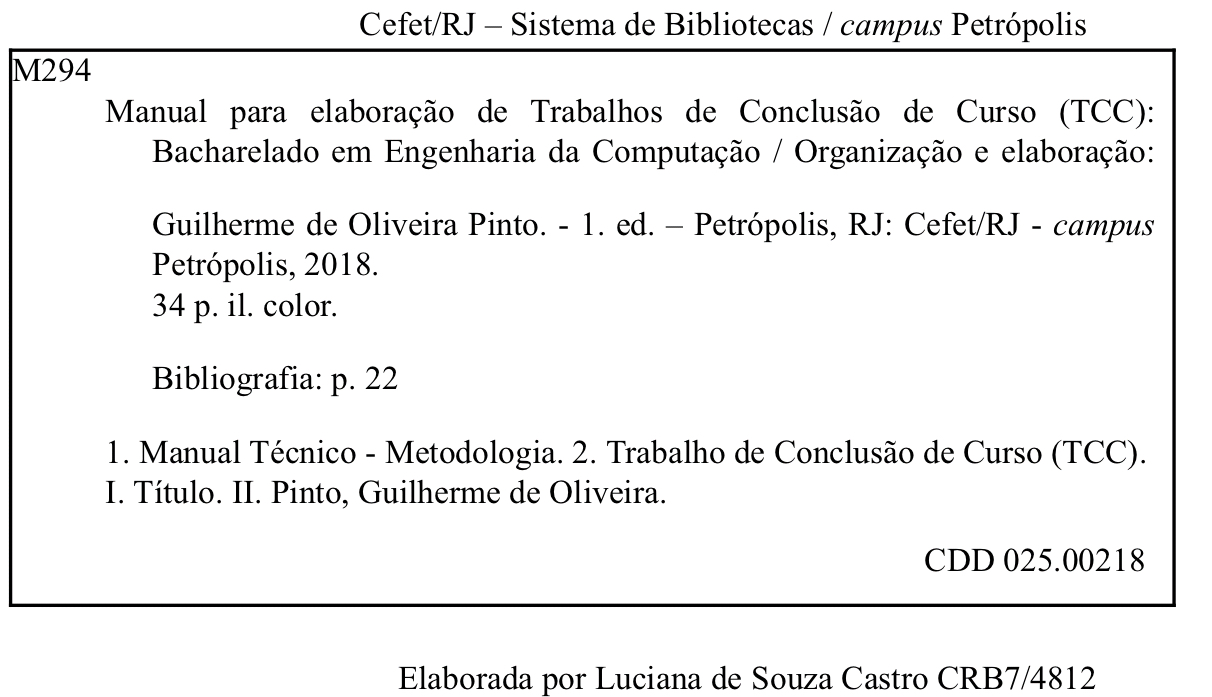
\includegraphics[height=0.4\textwidth]{Figs/biblioteca_engcomp.jpeg} 
\end{center}






%--------------------------------------------------------------------------
%--------------------------------------------------------------------------

\newpage
\newcommand{\HRule}{\rule{0.6\linewidth}{0.5mm}}
\pagestyle{empty}

{\center % Center everything on the page


\begin{figure}
\center

\includegraphics[height=0.13\textwidth]{Figs/logoCefetCampusPetropolis.jpg} 
\end{figure}

\begin{center}
{\large \bf CENTRO FEDERAL DE EDUCAÇÃO TECNOLÓGICA} \vspace{1mm} \\
{\large \bf CELSO SUCKOW DA FONSECA - CEFET/RJ \textit{CAMPUS} PETRÓPOLIS} \vspace{1mm} \\
{\large \bf CURSO: BACHARELADO EM ENGENHARIA DE COMPUTAÇÃO}\\
\vspace*{1.2cm}
{\large  FOLHA DE APROVAÇÃO}

\vspace*{1.3cm}
{\large \bf  Previsão Neural de Tendência de Valores Futuros do Bitcoin}\\
\end{center}
\vspace{0.5cm}
\hfill
%\begin{minipage}%{0.45\linewidth}
\begin{flushright}
    Bernardo Botelho Antunes da Costa
	\end{flushright}
%\end{minipage}
\vspace*{0.5cm}
\begin{flushright}
	\begin{minipage}{0.5\textwidth}
		{\normalsize
		Trabalho de Conclusão de Curso apresentado ao  
	 CEFET/RJ -{ {\it campus} Petrópolis}, como parte dos requisitos para obtenção do título de Bacharel em Engenharia de Computação.}
	\end{minipage}\\[0.5cm]
\end{flushright}
\vspace{0.5cm}
\hfill
%\begin{minipage}%{0.45\linewidth}
\begin{flushright}
Orientadora: Profa. Margaret Hamilton
\end{flushright}

\begin{minipage}{0.9\textwidth}
	\begin{flushleft}
	Aprovado por:
	\end{flushleft}
\end{minipage}\\[1cm]

\center
\HRule \\
Prof. Diego Barreto Haddad, D.Sc. (Orientador) \\[0.4cm]
\HRule \\
Prof. Luís Domingues Tomé Jardim Tarrataca, D.Sc.\\[0.4cm]
\HRule \\
Prof. Que o Diego escolher, D.Sc.  \\[1.5cm]


\begin{center}
{Agosto de 2018}
\end{center}


}



\newpage


% Dedicat�ria
%\begin{center}
%\textbf{\large DEDICATÓRIA}
%\end{center}
%      \vspace{0.5cm}
%
%Opcional.
%\newpage



% Agradecimento
\begin{center}
\textbf{\large  AGRADECIMENTO}
\end{center}
      \vspace{0.5cm}

Dedico este trabalho ao povo brasileiro que contribuiu de forma significativa a minha formação e estada nesta Universidade. Este projeto é uma pequena forma de retribuir o investimento e confiança em mim depositados.



\newpage


% Resumo
\begin{center}
\textbf{\large RESUMO}
\end{center}
      \vspace{0.5cm}

Inserir o resumo do seu trabalho aqui.

\begin{flushleft}
{\bf Palavras-chaves:} Previsão. Bitcoin. Google Trends. Redes neurais.
\end{flushleft}

\newpage

\begin{center}
\textbf{\large ABSTRACT}
\end{center}
\vspace{0.5cm}

Inserir o resumo do trabalho aqui, na Língua Inglesa.


\begin{flushleft}
{\bf Key-words:} Forecasting. Bitcoin. Google Trends. Neural Networks.
\end{flushleft}

\newpage

%=============================== lista de tabelas e figuras ==========================
{\thispagestyle{empty}
\renewcommand{\listfigurename}{LISTA DE FIGURAS}

\listoffigures}
\newpage

{\thispagestyle{empty}
\renewcommand{\listtablename}{LISTA DE TABELAS}
\listoftables}
\newpage

\begin{center}
\textbf{\large LISTA DE SIGLAS}
\end{center}
\vspace{0.5cm}
\singlespacing
\noindent
\begin{tabular}{l c p{.85\linewidth}}
CEFET & - & Centro Federal de Educação Tecnológica \\
TCC & - & Trabalho de Conclusão de Curso \\
PCA & - & Principal Component Analysis \\
AML & - & Amazon Machine Learning \\
ReLU & - & Rectified Linear Unit \\
MSE & - & Mean Square Error \\
BART & - & Bayesian Additive Regression Trees \\
DHC & - & District Heating and Cooling systems \\
ARIMA & - & Autoregressive Integrated Moving Average \\
DAEPF & - & Day-Ahead Electricity Price Forecasting \\
LSTM & - & Long Short Term Memory \\
BTC & - & Bitcoin \\
ETH & - & Ethereum \\
LTC & - & Litecoin \\
XRP & - & Ripple \\
BCH & - & Bitcoin Cash \\
API & - & Application Programming Interface \\
RNN & - & Rede Neurais Recorrentes \\
LSTM & - & Long Short-Term Memory \\
RMS & - & Root Mean Square \\
AWS & - & Amazon Web Services \\
EEM & - & European Energy Market \\
IEEE & - & Instituto de Engenheiros Eletricistas e Eletrônicos \\
ISSN & - & International Standard Serial Number \\
IGARSS & - & International Geoscience and Remote Sensing Symposium  \\
ISBI & - & International Symposium on Biomedical Imaging \\
IPTA & - & International Conference on Image Processing Theory, Tools and Applications \\
EHB & - & E-Health and Bioengineering Conference \\
EECS & - & European Conference on Electrical Engineering and Computer Science \\
ICSG & - & International Istanbul Smart Grids and Cities Congress and Fair \\
ISGT & - & Innovative Smart Grid Technologies \\
ICRIS & - & International Conference on Robots Intelligent System \\
CSUR & - & ACM Computing Surveys \\
\end{tabular}

\onehalfspacing

\newpage

%=============================== sum�rio =============================================

\tableofcontents

\newpage
%caso o sum�rio acabe em uma p�gina �mpar, o verso ser� em branco
%\null \vfill
%\newpage

%Agora muda para o estilo fancy
\pagestyle{fancy}
\pagenumbering{arabic}
\setcounter{page}{12}
\onehalfspacing

\newpage
Download


Source

PDF
Actions

   Copy Project
   Publish as Template
   Word Count
Sync

   Dropbox
   GitHub
   Mendeley
Settings

Compiler

Main document

Spell check

Auto-complete

Auto-close Brackets

Code check

Editor theme

Overall theme

Keybindings

Font Size

Font Family

Line Height

PDF Viewer

Hotkeys

   Show Hotkeys
Menu
TemplateTCC_VF_Bernardo
B
Review
Share
Submit
History
Chat
Browsing project as of 4th Nov 2018, 2:44 am
 Label this version Compare to another version Restore to before these changes
Show all of the project history or only labelled versions.All historyLabels
Figs
TCC.bcf
TCC.run.xml
TCC.lof
TCC.pdf
TCC.lot
Siglas.tex
TCC.tex
abnt-alf.bst
abnt.bst
abntex2.cls
abntex2abrev.sty
abntex2cite.sty
apateste.bst
apateste.bst.tex
apendiceA_TCC.tex
apendiceC_TCC.tex
apendiceNormas.tex
biblio.bib
bibliografia.bib
cap1.tex
cap3.tex
capaNew.tex
elsarticle-harv.bst
elsarticle.cls
model3-num-names.bst
model3-num-names11.bst.tex
model3-num-namesold.bst.tex
tocloft.sty
conclusao.tex
csv
Figuras
cap5.tex
cap4.tex
cap2.tex
Today
Edited cap1.tex
Edited cap2.tex
Edited cap4.tex
4:07 am • You
Edited cap1.tex
Edited cap2.tex
3:59 am • You
Edited bibliografia.bib
Edited cap1.tex
3:54 am • You
Edited bibliografia.bib
Edited cap2.tex
3:47 am • You
Edited bibliografia.bib
Edited cap1.tex
3:42 am • You
Edited cap1.tex
3:34 am • You
Edited cap1.tex
3:29 am • You
Edited cap2.tex
3:22 am • You
Edited cap2.tex
3:17 am • You
Edited cap2.tex
3:08 am • You
Edited cap2.tex
3:02 am • You
Edited bibliografia.bib
Edited cap4.tex
2:44 am • You
Edited bibliografia.bib
Edited cap3.tex
2:27 am • You
Edited bibliografia.bib
Edited cap4.tex
2:16 am • You
Edited bibliografia.bib
Edited cap2.tex
2:00 am • You
Edited cap2.tex
1:48 am • You
Edited cap2.tex
Edited cap4.tex
1:42 am • You
Edited cap2.tex
1:37 am • You
Edited cap2.tex
1:32 am • You
Edited cap2.tex
1:27 am • You
Yesterday
Edited cap4.tex
8:40 pm • karineribeiroc
Edited cap4.tex
8:34 pm • karineribeiroc
Edited cap4.tex
8:29 pm • karineribeiroc
Edited cap4.tex
8:20 pm • karineribeiroc
Edited cap4.tex
8:15 pm • karineribeiroc
Edited cap4.tex
8:06 pm • karineribeiroc
Edited cap4.tex
7:58 pm • karineribeiroc
Edited cap3.tex
7:52 pm • karineribeiroc
Edited cap2.tex
12:55 am • You
Edited cap2.tex
12:50 am • You
Edited cap1.tex
Edited cap2.tex
12:44 am • You
Edited biblio.bib
Edited bibliografia.bib
Edited cap1.tex
12:39 am • You
Edited biblio.bib
12:33 am • You
Deletedcap6.tex
12:24 am • You
Edited TCC.tex
Edited capaNew.tex
12:24 am • You
Edited capaNew.tex
12:18 am • You
Edited cap4.tex
Edited capaNew.tex
12:13 am • You
Edited cap4.tex
12:08 am • You
Yesterday
Edited cap4.tex
11:49 pm • You
Edited cap4.tex
11:43 pm • You
Edited cap4.tex
11:34 pm • You
Edited cap4.tex
11:27 pm • You
Edited cap4.tex
8:17 pm • You
Thu, 1st Nov 18
Edited cap3.tex
9:06 pm • karineribeiroc
Edited cap3.tex
6:14 pm • karineribeiroc
Edited cap2.tex
Edited cap3.tex
6:09 pm • karineribeiroc
Edited cap2.tex
6:04 pm • karineribeiroc
Edited cap2.tex
5:37 pm • karineribeiroc
Edited cap1.tex
4:20 pm • karineribeiroc
Edited cap1.tex
4:08 pm • karineribeiroc
Wed, 31st Oct 18
Edited cap1.tex
8:18 pm • karineribeiroc
Edited cap1.tex
8:10 pm • karineribeiroc
Tue, 30th Oct 18
Edited cap4.tex
11:55 pm • You
Edited cap4.tex
11:49 pm • You
Edited cap4.tex
11:35 pm • You
Edited cap4.tex
11:29 pm • You
Edited cap3.tex
Edited cap4.tex
11:22 pm • You
Edited cap4.tex
11:15 pm • You
Edited cap4.tex
11:08 pm • You
Edited cap4.tex
11:03 pm • You
Edited cap4.tex
12:15 am • You
Mon, 29th Oct 18
Edited cap4.tex
11:56 pm • You
Edited cap4.tex
11:50 pm • You
Edited cap4.tex
11:44 pm • You
Edited cap4.tex
11:38 pm • You
Edited cap4.tex
11:30 pm • You
Edited cap4.tex
11:25 pm • You
Edited cap4.tex
11:11 pm • You
Edited cap4.tex
11:06 pm • You
Edited TCC.tex
Edited cap4.tex
11:01 pm • You
Edited cap4.tex
10:55 pm • You
Edited cap4.tex
10:49 pm • You
Edited cap4.tex
10:40 pm • You
Edited cap4.tex
10:33 pm • You
Edited cap4.tex
10:28 pm • You
Edited cap4.tex
10:23 pm • You
Edited cap4.tex
10:17 pm • You
Edited cap4.tex
9:48 pm • You
Edited cap4.tex
9:39 pm • You
Edited TCC.tex
Edited cap4.tex
9:24 pm • You
Edited cap4.tex
9:02 pm • You
Edited cap4.tex
8:56 pm • You
Edited cap4.tex
8:51 pm • You
Edited TCC.tex
Edited cap4.tex
8:35 pm • You
RenamedCap2.tex → cap2.tex
RenamedCap4.tex → cap4.tex
RenamedCap5.tex → cap5.tex
RenamedCap6.tex → cap6.tex
8:30 pm • You
Edited TCC.tex
Edited biblio.bib
Edited bibliografia.bib
Edited capaNew.tex
8:30 pm • You
Edited TCC.tex
8:24 pm • You
Deletedteste.png
Deletedrsz_tom_cruise.png
Deletedrsz_image.png
Deletedlstm_chain.png
DeletedLSTM3-SimpleRNN.png
Deletedgrafico.png
DeletedFigure_1.png
Deletedcodigo_treinar.py
CreatedFiguras/Cap2/neuronio.png
Createdcsv/bitcoin_coindesk_12m.csv
Createdcsv/ethereum_coindesk_12m.csv
Createdcsv/bcash_gtrends_12m.csv
Createdcsv/bcash_investing_12m.csv
Createdcsv/ripple_gtrends_12m.csv
Createdcsv/1d.csv
Createdcsv/gt.csv
Createdcsv/price_n.csv
Createdcsv/bitcoin_gtrends_12m.csv
Createdcsv/ethereum_gtrends_12m.csv
Createdcsv/litecoin_coinmarketcap_12m.csv
Createdcsv/price.csv
Createdcsv/2d.csv
Createdcsv/gt_n.csv
Createdcsv/ripple_investing_12m.csv
Createdcsv/litecoin_gtrends_12m.csv
DeletedFiguras/csv/bitcoin_coindesk_12m.csv
DeletedFiguras/csv/ethereum_coindesk_12m.csv
DeletedFiguras/csv/bcash_investing_12m.csv
DeletedFiguras/csv/ripple_gtrends_12m.csv
DeletedFiguras/csv/gt.csv
DeletedFiguras/csv/price_n.csv
DeletedFiguras/csv/bitcoin_gtrends_12m.csv
DeletedFiguras/csv/ethereum_gtrends_12m.csv
DeletedFiguras/csv/litecoin_coinmarketcap_12m.csv
DeletedFiguras/csv/price.csv
DeletedFiguras/csv/gt_n.csv
DeletedFiguras/csv/ripple_investing_12m.csv
DeletedFiguras/csv/litecoin_gtrends_12m.csv
DeletedFiguras/csv/neuronio.png
DeletedFiguras/csv/bcash_gtrends_12m.csv
DeletedFiguras/csv/2d.csv
DeletedFiguras/csv/1d.csv
RenamedFiguras/bitcoin_coindesk_12m.csv → Figuras/csv/bitcoin_coindesk_12m.csv
RenamedFiguras/ethereum_coindesk_12m.csv → Figuras/csv/ethereum_coindesk_12m.csv
RenamedFiguras/bcash_investing_12m.csv → Figuras/csv/bcash_investing_12m.csv
RenamedFiguras/ripple_gtrends_12m.csv → Figuras/csv/ripple_gtrends_12m.csv
RenamedFiguras/gt.csv → Figuras/csv/gt.csv
RenamedFiguras/price_n.csv → Figuras/csv/price_n.csv
RenamedFiguras/bitcoin_gtrends_12m.csv → Figuras/csv/bitcoin_gtrends_12m.csv
RenamedFiguras/ethereum_gtrends_12m.csv → Figuras/csv/ethereum_gtrends_12m.csv
RenamedFiguras/litecoin_coinmarketcap_12m.csv → Figuras/csv/litecoin_coinmarketcap_12m.csv
RenamedFiguras/price.csv → Figuras/csv/price.csv
RenamedFiguras/gt_n.csv → Figuras/csv/gt_n.csv
RenamedFiguras/ripple_investing_12m.csv → Figuras/csv/ripple_investing_12m.csv
RenamedFiguras/litecoin_gtrends_12m.csv → Figuras/csv/litecoin_gtrends_12m.csv
RenamedFiguras/neuronio.png → Figuras/csv/neuronio.png
RenamedFiguras/bcash_gtrends_12m.csv → Figuras/csv/bcash_gtrends_12m.csv
RenamedFiguras/2d.csv → Figuras/csv/2d.csv
RenamedFiguras/1d.csv → Figuras/csv/1d.csv
CreatedFiguras/bitcoin_coindesk_12m.csv
CreatedFiguras/ethereum_coindesk_12m.csv
CreatedFiguras/bcash_gtrends_12m.csv
CreatedFiguras/bcash_investing_12m.csv
CreatedFiguras/ripple_gtrends_12m.csv
CreatedFiguras/1d.csv
CreatedFiguras/gt.csv
CreatedFiguras/price_n.csv
CreatedFiguras/bitcoin_gtrends_12m.csv
CreatedFiguras/ethereum_gtrends_12m.csv
CreatedFiguras/litecoin_coinmarketcap_12m.csv
CreatedFiguras/price.csv
CreatedFiguras/2d.csv
CreatedFiguras/gt_n.csv
CreatedFiguras/ripple_investing_12m.csv
CreatedFiguras/litecoin_gtrends_12m.csv
CreatedFiguras/neuronio.png
8:21 pm • You
Deletedarticle_cite/Capturar1.PNG
Deletedarticle_cite/Capturar.PNG
Deletedarticle_cite/Capturar4.PNG
Deletedarticle_cite/Capturar3.PNG
Deletedarticle_cite/Capturar2.PNG
8:15 pm • You
Edited Cap2.tex
Edited Cap4.tex
Edited Cap5.tex
Edited Cap6.tex
Edited cap1.tex
Edited cap3.tex
8:14 pm • You
Createdconclusao.tex
CreatedCap6.tex
CreatedCap5.tex
CreatedCap4.tex
CreatedCap2.tex
Createdtocloft.sty
Createdmodel3-num-namesold.bst.tex
Createdmodel3-num-names11.bst.tex
Createdmodel3-num-names.bst
Createdelsarticle.cls
Createdelsarticle-harv.bst
CreatedcapaNew.tex
Createdcap3.tex
Createdcap1.tex
Createdbibliografia.bib
Createdbiblio.bib
CreatedapendiceNormas.tex
CreatedapendiceC_TCC.tex
CreatedapendiceA_TCC.tex
Createdapateste.bst.tex
Createdapateste.bst
Createdabntex2cite.sty
Createdabntex2abrev.sty
Createdabntex2.cls
Createdabnt.bst
Createdabnt-alf.bst
CreatedTCC.tex
CreatedSiglas.tex
CreatedLSTM3-SimpleRNN.png
Createdlstm_chain.png
CreatedTCC.lot
CreatedTCC.pdf
Createdcodigo_treinar.py
Createdrsz_tom_cruise.png
Createdrsz_image.png
Createdteste.png
Createdgrafico.png
CreatedTCC.lof
CreatedTCC.run.xml
CreatedFigure_1.png
CreatedTCC.bcf
Createdarticle_cite/Capturar1.PNG
Createdarticle_cite/Capturar.PNG
Createdarticle_cite/Capturar4.PNG
Createdarticle_cite/Capturar3.PNG
Createdarticle_cite/Capturar2.PNG
CreatedFigs/logoEngComp.png
CreatedFigs/logoCefetCampusPetropolis-eps-converted-to.pdf
CreatedFigs/biblioteca.jpeg
CreatedFigs/logoEngComp.eps
CreatedFigs/republica.eps
CreatedFigs/republica.png
CreatedFigs/pedestres.jpg
CreatedFigs/logoCefetCampusPetropolis.eps
CreatedFigs/biblioteca_engcomp.jpeg
CreatedFigs/logoCefetRio.eps
CreatedFigs/logoCefetCampusPetropolis.jpg
CreatedFigs/logo.PNG
CreatedFigs/logoCefetRio-eps-converted-to.pdf
8:13 pm • You

1
2
3
4
5
6
7
8
9
10
11
12
13
14
15
16
17
18
19
20
21
22
23
\section{Introduçao}
 \subsection{Séries Temporais}
 \label{sec:SeriesTemporais}
Séries temporais são definidas como ``qualquer conjunto de observações ordenadas no tempo'' 
    \cite{morettin2006analise}. Elas são observadas em problemas envolvendo diversas áreas de 
    conhecimento, tais como: meteorologia \cite{7982030}, processamento de imagens 
    \cite{7729869,7164182, 6723283}, processamento de vídeos \cite{6469509}, marca d'água 
    digital\footnote{\textit{Digital watermarking} - ou, em português, marca d'água digital é 
    uma técnica esteganográfica de ocultação de informação.} \cite{7024611}, agricultura 
    \cite{6723610}, medicina \cite{6707296} economia \cite{4810671}, entre outros.
 
 \subsection{Tipos de Séries Temporais}
 Existem séries temporais \textit{discretas} e \textit{contínuas}. As discretas costumam ser 
     obtidas através de amostragem de uma série contínua a intervalos de tempo regulares 
     \cite{morettin2006analise,hyndman2018forecasting}. Por exemplo, para analisar a série do 
     valor da temperatura de uma cidade ao longo de um ano, será preciso amostrá-la a 
     intervalos, obtendo uma lista de valores. Esse processo converte uma série contínua em uma 
     série discreta.
Os estudos de séries temporais estão geralmente relacionados a dois domínios: o domínio do 
    tempo e o domínio da frequência. Ambos os enfoques estão interessados em construir modelos 
    para séries. Os modelos no domínio do tempo em geral são paramétricos, ou seja, têm um 
    número finito de parâmetros \cite{conover1981rank}. Já os modelos no domínio da frequência 
    são classificados como não-paramétricos \cite{hollander1999nonparametric}. Em termos mais 
    rigorosos, modelos paramétricos são aqueles que assumem um conjunto finito de parâmetros 
    que cumpre estimar, o que limita a complexidade do modelo mesmo quando a informação contida 
    nos dados é arbitrariamente grande. Já os modelos não paramétricos assumem que a 
    distribuição dos dados depende de um conjunto de parâmetros de dimensionalidade infinita. 
    Estes modelos capturam mais informação dos dados à medida que a disponibilidade de 
    informação aumenta, o que os torna mais flexíveis \cite{ChenNeural2001}.
 
\subsection{Notação}
Este trabalho interpretará uma série temporal como um vetor, cujos elementos consistem de 
    amostras no tempo $t$. Admitindo um total de $r$ elementos, podemos definir o vetor 
    $\boldsymbol{z}(t) \in \mathbb{R}^n$ que contém uma série temporal como
\begin{equation}
\boldsymbol{z}(t) \triangleq \begin{bmatrix}z(t_1) & z(t_2) & \ldots & z(t_n)\end{bmatrix}.
\end{equation}
%\dbh{Prefiro a seguinte notação: vetores em negrito e minúsculas, escalares em fonte normal e 
    matrizes em negrito e em maiúsculas}.
 
 \subsection{Estacionariedade}
 
 Uma série temporal é dita estacionária de primeira ordem quando se desenvolve no tempo 
     aleatoriamente ao redor de uma média constante. A maioria dos procedimentos de análise 
     estatística de séries temporais supõe que estas sejam estacionárias. Caso tal hipótese não 
     se confirme, será necessário efetuar alguma transformação nos dados originais de sorte a 
     realçar a estacionariedade da série transformada \cite{grenander1957statistical}.
 A transformação mais comum consiste em tomar diferenças sucessivas da série original. Esta 
     técnica é conhecida como diferenciação. Seu objetivo consiste em ajudar a estabilizar a 
     média de uma série temporal, removendo as alterações bruscas no nível de uma série 
     temporal e, portanto, eliminando (ou reduzindo) a tendência e a sazonalidade 
     \cite{morettin2006analise, hyndman2018forecasting}.

\section{Redes Neurais}
\subsection{O que são Redes Neurais?}
\label{subsec:oquesaoredesneurais}

As redes neurais artificiais, como conhecidas na literatura \cite{haykin2004comprehensive, haykin2009neural, lecun2015deep}, são estruturas aptas ao aprendizado inspiradas na forma com que os neurônios de cérebros reais funcionam. Um modo estrutural de organização, bem como a distribuição de informação ao longo da arquitetura foram levados em conta na construção deste poderoso modelo matemático que hoje conhecemos como Redes Neurais \cite{haykin2004comprehensive, haykin2009neural, lecun2015deep}. Tais redes são reconhecidamente uma tecnologia bioinspirada, já que são profundamente motivadas pelo aprendizado demonstrado pelo cérebro de seres vivos, notadamente o dos seres humanos. 
\begin{figure}[b]
    \centering
    \caption{Representação de um neurônio.}
    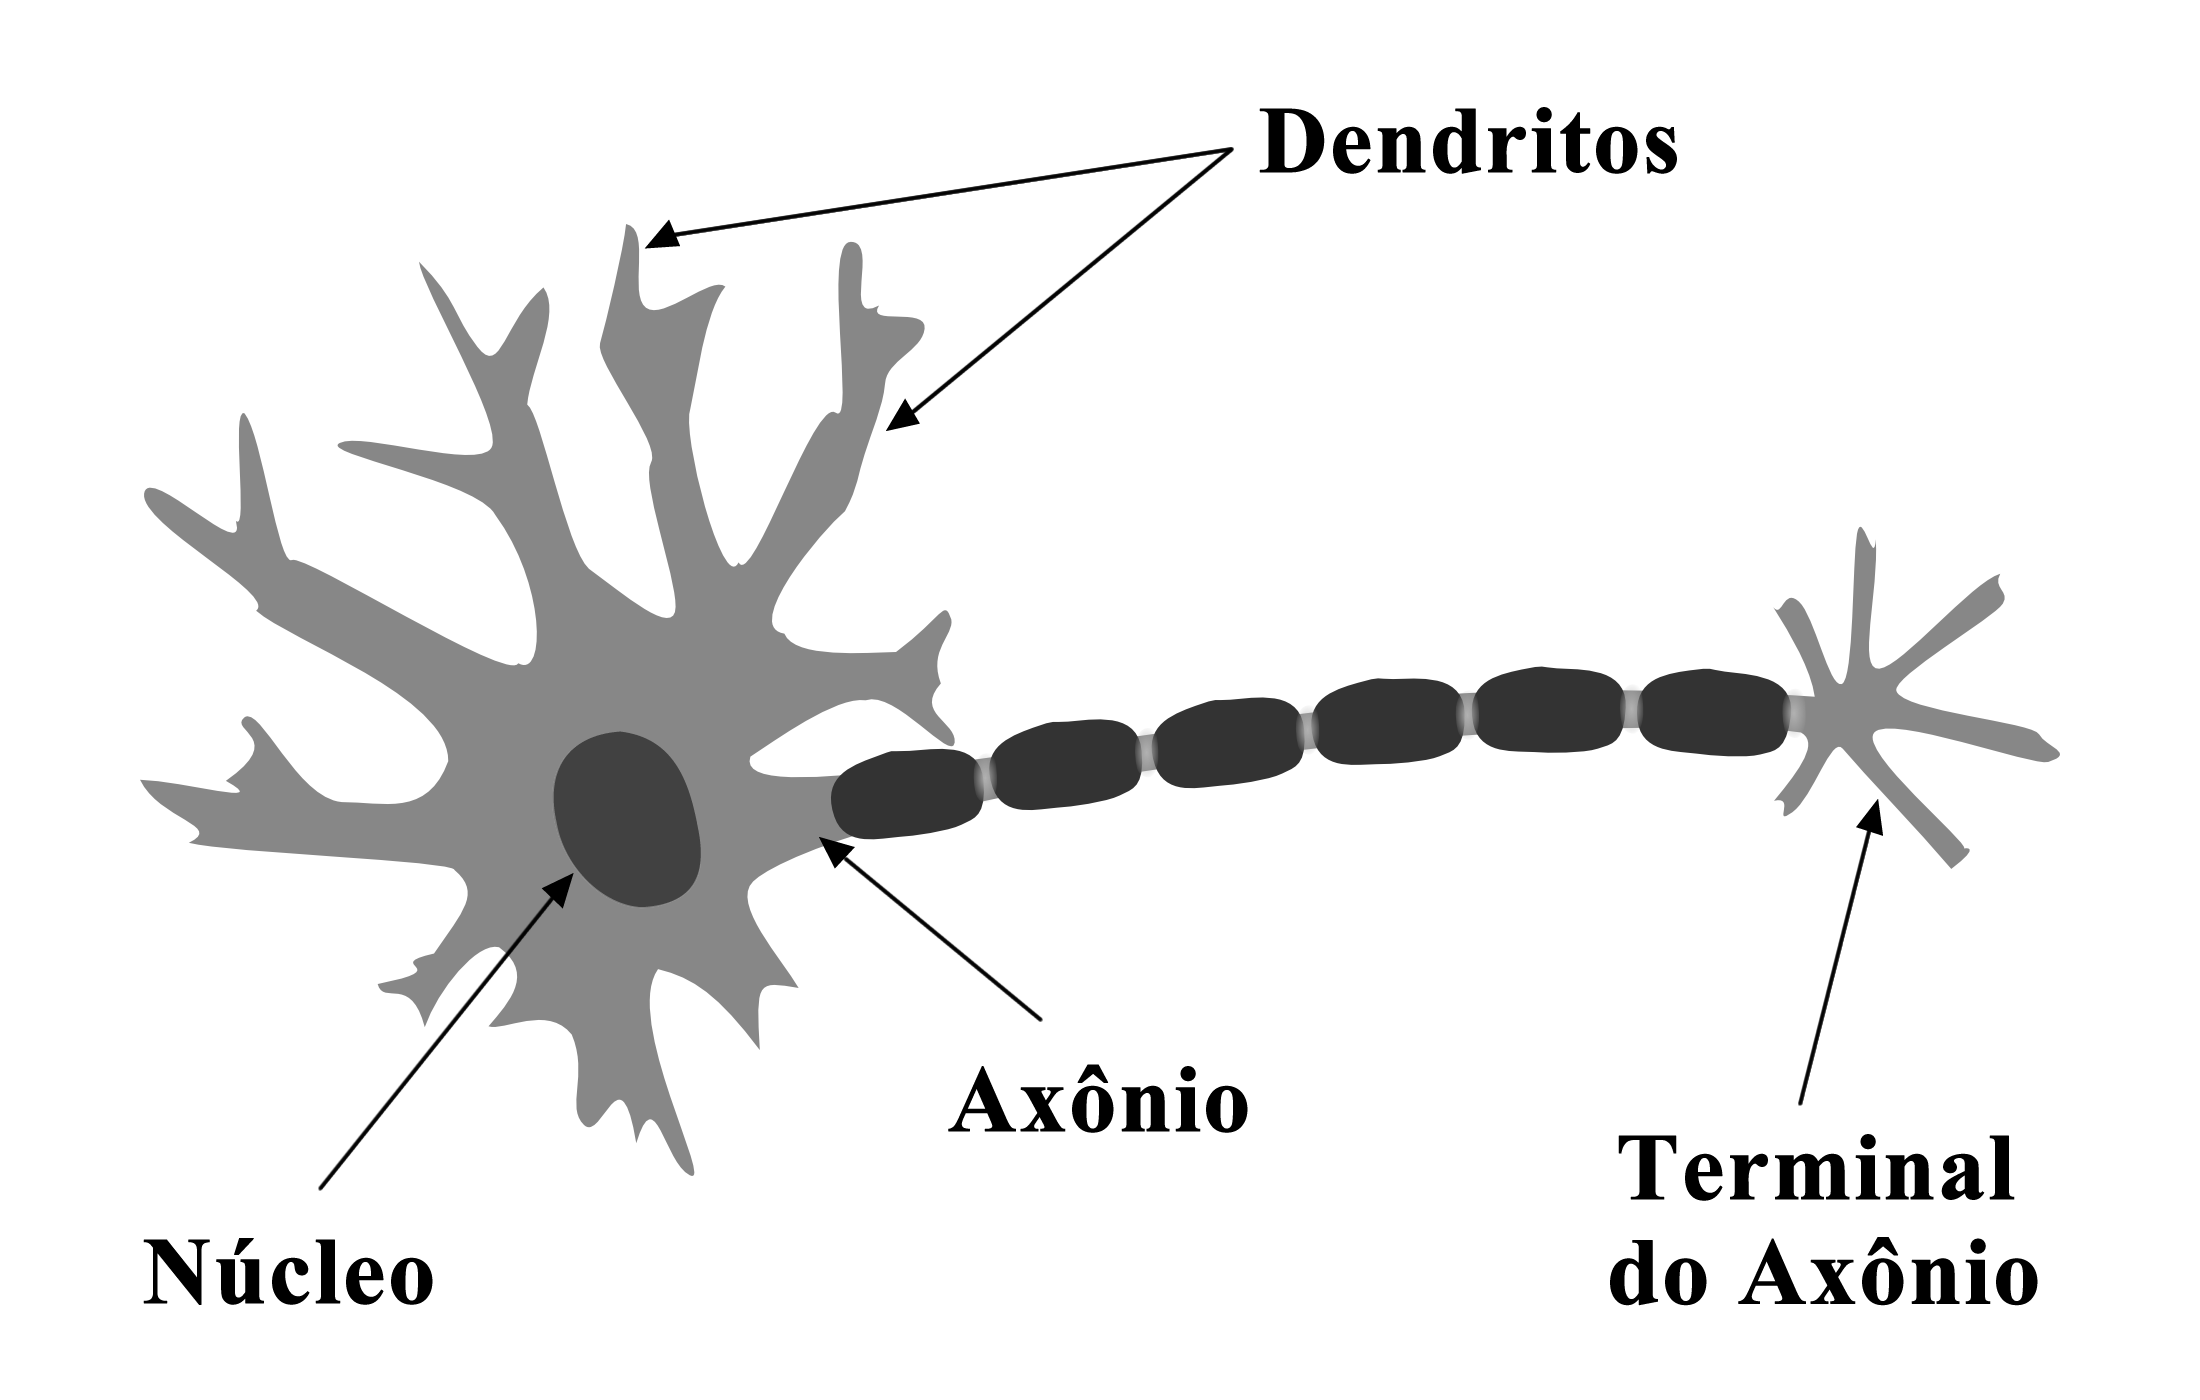
\includegraphics[scale=0.17]{Figuras/Cap2/neuronio.png}
    \begin{center}
    Fonte:
        Figura \ref{fig:neuronio} extraída do site Pixabay \cite{Pixabay} e editada pelo autor. O site Pixabay \cite{Pixabay} é uma plataforma gratuita de distribuição de imagens, ou seja, o uso das imagens não ferem direitos autorais.
    \end{center}
         
        \label{fig:neuronio}
\end{figure}


A Figura \ref{fig:neuronio} representa um neurônio utilizado como componente fundamental das redes neurais artificiais. Para entender como essa representação nos leva ao modelo matemático, devemos primeiro descrever suas quatro partes principais, bem como a função de cada parte do neurônio.

\begin{enumerate}
    \item núcleo: onde é processada a informação;
    \item dendrito: de onde vem a informação a ser processada (ou seja, o \textit{input});
    \item axônio: parte que o neurônio usa para enviar sinais (ou seja, o \textit{output});
    \item terminal do axônio: onde a informação de saída é propagada para os demais neurônios da rede ou utilizada como resposta final da rede.
\end{enumerate}

Uma rede neural artificial é implementada por meio da conexão de diversos neurônios, cujos axônios se conectam ao dendritos de outro, levando o sinal processado pelo núcleo. Os neurônios recebem tal sinal em seus dendritos os quais, por sua vez, processam o sinal em seus núcleos, enviando novamente o resultado (via axônios) para os próximos neurônios, por meio dos terminais dos axônios. Eis a lógica de propagação e processamento de informação que as redes neurais artificiais almejam emular.

Este trabalho tem como motivação o uso de Redes Neurais pelos benefícios que elas trazem para o problema específico da previsão de valores do Bitcoin. A motivação biológica não faz parte das motivações deste trabalho.

A próxima subseção apresentará a representação gráfica e matemática de uma Rede Neural, que será usada no decorrer deste trabalho.

\subsection{Representação de uma Rede Neural}

\subsubsection{Representação de um Neurônio}
\label{subsubsec:representacaoumneuronio}

No objetivo de representar mais formalmente o processamento matemático empreendido por uma Rede Neural, vamos transformar as quatro principais partes do neurônio da subseção \ref{subsec:oquesaoredesneurais} em um diagrama. A Figura \ref{fg:rede_neural_simples} apresenta o diagrama de um neurônio, no qual podemos elencar os componentes seguintes:
\begin{enumerate}
 \item dendrito (\textit{input}): representado pelos círculos azuis. Cada círculo contém o valor referente à sua amostra $x_n$; nesse exemplo, $n = 3$ amostras. A informação de cada uma das $n$ amostras é enviada para o núcleo;
    \item núcleo: representado pelo círculo laranja. No núcleo, as amostras $x_n$ e os pesos $\theta_n$ executam a chamada \textbf{função de ativação}, apresentada na Seção \ref{sec:funcaoativacao};
   
    \item axônio (\textit{output}): consiste na saída do núcleo, a qual armazena o resultado da operação;
    \item terminal do axônio: descreve a transformação da saída num (\textit{input}) de um novo neurônio, geralmente da camada posterior.
    
\end{enumerate}


\begin{figure}
\centering
\caption{Representação de um neurônio}
\large
\begin{tikzpicture}[shorten >=1pt,->,draw=black!70, node distance=\layersep]
    \tikzstyle{every pin edge}=[<-,shorten <=1pt]
    \tikzstyle{neuron}=[circle,fill=black!50,minimum size=05pt,inner sep=15pt]
    \tikzstyle{input neuron}=[neuron, fill=blue!50];
    \tikzstyle{output neuron}=[neuron, fill=orange!50, inner sep=10pt];

    \tikzstyle{annot} = [text width=4em, text centered]

    % Draw the input layer nodes
    \foreach \name \y in {1,...,3}
        \node[input neuron, pin=left:] (I-\name) at (0,-2.2*\y){x\y};

    % Draw the output layer node
    \node[output neuron,pin={[pin edge={->}]right:}] (ou) at (3,-4.4) {$h\theta (x)$};

    % Connect every node in the hidden layer with the output layer
    \foreach \source in {1,...,3}
        \path (I-\source) edge (ou);

    % Annotate the layers
   \node[annot,above of=I-1, node distance=1.7cm] (hl) {Entrada};
   \node[annot] at (3, -0.5){Saída};
    
\end{tikzpicture}
\label{fg:rede_neural_simples}
\end{figure}

Os elementos desse neurônio podem ser escritos na forma matricial. Assumindo uma entrada $x$ composta de $n$ elementos, podemos representá-la como:
\begin{equation}
  \mathbf{x}^T \triangleq \begin{bmatrix}x_{1}&x_{2}&x_{3}&...&x_{n-1}&x_{n} \end{bmatrix}
\end{equation}
 com os pesos representados como:
 \begin{equation}
  \mathbf{\theta}^T \triangleq \begin{bmatrix}\theta_{1}&\theta_{2}&\theta_{3}&...&\theta_{n-1}&\theta_{n}\end{bmatrix}
\end{equation}

Frequentemente na literatura \cite{haykin2004comprehensive, haykin2009neural, lecun2015deep} é adicionado em cada neurônio uma amostra extra, chamada de \textit{bias}, ou viés. O \textit{bias} serve para aumentar os graus de liberdade do sistema, levando o resultado do Neurônio para uma determinada direção. Ele permite que restrições muito severas não sejam aplicadas ao sistema. Por exemplo, caso as entradas sejam nulas, o neurônio terá uma saída também nula, o que comumente é uma restrição muito forte. O  \textit{bias}, portanto,  permite uma melhor adaptação do sistema.

%FEITO
%\dbh{Errado, Bernardo! Esse bias é essencial, porque caso contrário a rede neural necessariamente irá jogar uma entrada nula numa saída também nula, o que comumente é uma restrição muito forte!!!}

\subsubsection{Representação de uma Rede Neural}
\label{subsubsec:representacaoumaredeneural}
Nas seção \ref{subsubsec:representacaoumneuronio} foi apresentado a representação de um Neurônio. Nesta seção, será empregada a representação da seção anterior para definir uma Rede Neural, que será usada como modelo no restante deste trabalho. A expansão da representação de \ref{subsubsec:representacaoumneuronio} permite uma descrição global de uma rede neural artificial. A Figura \ref{fg:rede_neural_generica} representa uma Rede Neural. Essa rede possui $n$ componentes de entrada, $m$ neurônios em cada uma das $k$ camadas, onde $n, m, k\in \mathbb{N}$. Cada neurônio aplica uma função não linear nas entradas que recebe; normalmente tal função pode ser a sigmoidal (\ref{subsec:sigmoid}), a tangente hiperbólica (\ref{subsec:htan}) ou a ReLu (\ref{subsec:relu}), que serão abordadas especificamente na seção \ref{sec:funcaoativacao}.

%--

\begin{figure}
\centering
\caption{Representação de uma Rede Neural}
\large
\begin{tikzpicture}[shorten >=1pt,->,draw=black!50, node distance=\layersep]
    \tikzstyle{every pin edge}=[<-,shorten <=1pt]
    \tikzstyle{neuron}=[circle,fill=black!25,minimum size=17pt,inner sep=15pt]
    \tikzstyle{input neuron}=[neuron, fill=blue!50];
    \tikzstyle{output neuron}=[neuron, fill=orange!50,inner sep=13pt];
    \tikzstyle{hidden neuron}=[neuron, fill=red!50,inner sep=13pt];
     \tikzstyle{hidden_n neuron}=[neuron, fill=red!30,inner sep=10pt];
     \tikzstyle{p neuron}=[neuron, fill=red!40,inner sep=17pt];
    \tikzstyle{annot} = [text width=4em, text centered]
    
    \node[input neuron, pin=left:] (I-1) at (-5,-2.2*1) {$x_1$};
    \node[input neuron, pin=left:] (I-2) at (-5,-2.2*2) {$x_2$};
    \node[input neuron, pin=left:] (I-3) at (-5,-2.2*3) {$x_3$};
    \node[input neuron, pin=left:] (I-4) at (-5,-2.2*4) {...};
    \node[input neuron, pin=left:] (I-5) at (-5,-2.2*5) {$x_n$};
    
    \node[hidden neuron] (H-1) at (-2,-2.2*1) {$a_1^2$};
    \node[hidden neuron] (H-2) at (-2,-2.2*2) {$a_2^2$};
    \node[hidden neuron] (H-3) at (-2,-2.2*3) {$a_3^2$};
    \node[hidden neuron] (H-4) at (-2,-2.2*4) { ... };
    \node[hidden neuron] (H-5) at (-2,-2.2*5) {$a_m^2$};
    
    \node[p neuron] (p-1) at (1,-2.2*1) { ... };
    \node[p neuron] (p-2) at (1,-2.2*2) { ... };
    \node[p neuron] (p-3) at (1,-2.2*3) { ... };
    \node[p neuron] (p-4) at (1,-2.2*4) { ... };
    \node[p neuron] (p-5) at (1,-2.2*5) { ... };

    \node[hidden_n neuron] (Hn-1) at (4,-2.2*1) {$a_1^{k-1}$};
    \node[hidden_n neuron] (Hn-2) at (4,-2.2*2) {$a_2^{k-1}$};
    \node[hidden_n neuron] (Hn-3) at (4,-2.2*3) {$a_3^{k-1}$};
    \node[hidden_n neuron] (Hn-4) at (4,-2.2*4) { ... };
    \node[hidden_n neuron] (Hn-5) at (4,-2.2*5) {$a_{m}^{k-1}$};
    
    \node[output neuron,pin={[pin edge={->}]right:}] (O-1) at (7,-2.2*1) { $h_{\theta_1}$};
    \node[output neuron,pin={[pin edge={->}]right:}] (O-2) at (7,-2.2*2) { $h_{\theta_2}$};
    \node[output neuron,pin={[pin edge={->}]right:}] (O-3) at (7,-2.2*3) { $h_{\theta_3}$};
    \node[output neuron,pin={[pin edge={->}]right:}] (O-4) at (7,-2.2*4) { ... };
    \node[output neuron,pin={[pin edge={->}]right:}] (O-5) at (7,-2.2*5) { $h_{\theta_m}$};
    
    \foreach \source in {1,...,5}
        \foreach \dest in {1,...,5}
            \path (I-\source) edge (H-\dest);

    \foreach \source in {1,...,5}
        \foreach \dest in {1,...,5}
            \path (H-\source) edge (p-\dest);
            
    \foreach \source in {1,...,5}
        \foreach \dest in {1,...,5}
            \path (p-\source) edge (Hn-\dest);
    
    \foreach \source in {1,...,5}
        \foreach \dest in {1,...,5}
            \path (Hn-\source) edge (O-\dest);

    \node[annot] at (-5,-0.5) {Entradas};
    \node[annot] at (-2,-0.5){Camada 1};
    \node[annot] at (1, -0.5){...};
    \node[annot] at (4, -0.5){Camada k-1};
    \node[annot] at (7, -0.5){Camada k};
\end{tikzpicture}
\label{fg:rede_neural_generica}
\end{figure}


Para representar a Rede Neural, primeiramente, é preciso  representar $a^{(x)}_y$, que é chamada de \textbf{ativação}. A ativação é individual para cada Neurônio, onde $a^{(x)}_y$ é a ativação referente ao Neurônio da camada $x$, ficando a cargo de $y$ identificar o Neurônio dentro de todos os possíveis Neurônios da camada $x$. A \textbf{ativação} é calculado realizando a soma de todas as entradas de determinado Neurônio, multiplicadas pelos seus respectivos pesos, que servem de entrada para a função de ativação, que é o resultado do Neurônio em questão. Feito esse processo, podemos representar $a^{(x)}_y$ usando a equação \ref{fun:axy}.
\begin{equation}
    a^{(x)}_y=g(\Theta^{(x-1)}_{y0}x{}_0+\Theta^{(x-1)}_{y1}x{}_1+\Theta^{(x-1)}_{y2}x{}_2\Theta^{(x-1)}_{y3}x{}_3+...+\Theta^{(x-1)}_{y(m-1)}x{}_{m-1}+\Theta^{(x-1)}_{ym}x{}_m )
    \label{fun:axy}
\end{equation}


Sabendo como calcular os $a^{(x)}_y$ de todas as camadas, deixando claro que é preciso saber o resultado da camada anteriora para calcular a camada atual, é possível definir uma saída genérica $\mathbf{h}{\Theta}(x)_y$ como na  Eq. \ref{fun:thetanm}. Note que a Eq. \ref{fun:thetanm} é apenas consequência de ir executando a Eq.  \ref{fun:axy} até a última camada. Esse procedimento é conhecido como \textit{Forward Propagagtion}, e será abordado melhor na seção \ref{subsec:backpropagation} ao falar de Backpropagation.

\begin{equation}
    \mathbf{h}{\Theta}(x) = a^{(n)}_y = g(\Theta^{n-1}_{y0}a^{n-1}_{0}+\Theta^{n-1}_{y1}a^{n-1}_{1}+\Theta^{n-1}_{y2}a^{n-1}_{2}+...+\Theta^{n-1}_{y(n-1)}a^{n-1}_{n-1}+\Theta^{n-1}_{yn}a^{n-1}_{m})
     \label{fun:thetanm}
\end{equation}


Para simplificar os cálculos, é usual utilizar operações matriciais, que conseguem atualizar todos os seus componentes em uma única operação. Para representar todas as entradas, por exemplo, foi utilizado a Eq. \ref{fun:entrada_generica}.
%FEITO
%\dbh{O texto está muito seco; só definições matemáticas, as quais não apelam à intuição!}


\begin{equation}
    \label{fun:entrada_generica}
  \mathbf{x}^T = \begin{bmatrix}x_{1}&x_{2}&x_{3}&...&x_{n-1}&x_{n}\end{bmatrix}
\end{equation}

E a resposta da Rede Neural Genérica pode ser escrita na forma matricial mediante o emprego de \eqref{fun:h_generica}.

 \begin{equation}
   \label{fun:h_generica}
   \mathbf{h}\theta(x) = 
   \begin{bmatrix}
   g(\Theta^{(n-1)}_{10}a^{(n-1)}_{0}+\Theta^{(n-1)}_{11}a^{(n-1)}_{1}+ ... +\Theta^{(n-1)}_{1(m-1)}a^{(n-1)}_{(m-1)} )\\
   g(\Theta^{(n-1)}_{20}a^{(n-1)}_{0}+\Theta^{(n-1)}_{21}a^{(n-1)}_{1}+ ... +\Theta^{(n-1)}_{2(m-1)}a^{(n-1)}_{(m-1)} )\\
   g(\Theta^{(n-1)}_{30}a^{(n-1)}_{0}+\Theta^{(n-1)}_{31}a^{(n-1)}_{1}+ ... +\Theta^{(n-1)}_{3(m-1)}a^{(n-1)}_{(m-1)} )\\
    \vdots\\
    g(\Theta^{(n-1)}_{(m-1)0}a^{(n-1)}_{0}+\Theta^{(n-1)}_{(m-1)1}a^{(n-1)}_{1}+ ... +\Theta^{(n-1)}_{(m-1)}a^{(n-1)}_{(m-1)} )\\
    
   \end{bmatrix} 
\end{equation}


Essas são as representações gráficas e matemáticas que serão utilizadas no decorrer deste trabalho. Na próxima subseção será abordada a função de ativação.

\subsection{Funções de Ativação}
\label{sec:funcaoativacao}

\cite{activationfun}

\dbh{Motivar o emprego da função não-linear; a não linearidade é muito importante para o poder das redes neurais.}

\bac{motivar mais as funcoes de ativacao **ReLU copiada do guilherme}

A função de ativação é denotada como $h_\Theta (x)$ e define a saída de um neurônio para uma dada entrada $x$. Descreveremos a seguir a função de ativação sigmoide, a mais comum em Redes Neurais \cite{haykin2004comprehensive, haykin2009neural, lecun2015deep}.

\subsubsection{Função Sigmoide}
\label{subsec:sigmoid}
\dbh{Não, mil vezes não! A sigmoide é suave, não é brusca como mostrado na equação (23)! Este capítulo tem que ser muito lapidado. Só tem definições matemáticas, com pouca discussão motivadora! Ler mais!}

A Eq.\ref{fun:sigmoid} representa a função sigmoide, apresentada graficamente na Fig. \ref{fg:funcao_sigmoide}. 


\begin{equation}
  f(x) =  \frac{\mathrm{1} }{\mathrm{1} + e^{- \mathbf{\theta^T}x}}
  \label{fun:sigmoid}
\end{equation}

\begin{center}
    \begin{figure}
     \caption{Função Sigmoide}
        \centering
        \begin{tikzpicture}
        	\begin{axis}[
        		xlabel=$x$,
        		ylabel={$f(x)$}
        	]
        	\addplot {1 / (1 + e^-x)};
        	\end{axis}
        \end{tikzpicture}
   \label{fg:funcao_sigmoide}
	\end{figure}
\end{center}

\subsubsection{Função Tangente Hiperbólica}
\label{subsec:htan}
\bac{TANGENTE HIPERBOLCIA}

\begin{equation}
  f(x) =  \frac{\mathrm{1} - e^{- \mathbf{\theta^T}x}}{\mathrm{1} + e^{- \mathbf{\theta^T}x}}
  \label{fun:tanh}
\end{equation}

\begin{center}
    \begin{figure}
    \caption{Função Tangente Hiperbólica}
        \centering
        \begin{tikzpicture}
        	\begin{axis}[
        		xlabel=$x$,
        		ylabel={$f(x)$}
        	]
        	\addplot {(e^x - e^-x) / (e^x + e^-x)};
        	\end{axis}
        \end{tikzpicture}
    \label{fg:funcao_tanh}
	\end{figure}
\end{center}



\subsubsection{Função ReLU}
\label{subsec:relu}
A função ReLU (\textit{rectified linear unit}) realiza a ativação do nó apenas se a entrada estiver acima de um valor predeterminado. O ReLU é representado pela equação $\phi (x) = max(0,x)$. A Figura \ref{fig:relu} mostra o gráfico dessa função. Trata-se de uma função não linear (ainda que linear por partes) que permite implementações com baixo custo computacional.

\begin{figure}[!htb]
    \centering
    \caption{Função ReLU.}
    \begin{tikzpicture}
    \begin{axis}[
        		xlabel=$x$,
        		ylabel={$f(x)$}
        	]
        \addplot+[mark=none,blue,domain=-3:0] {0};
        \addplot+[mark=none,blue,domain=0:4] {x};
    \end{axis}
\end{tikzpicture}
\label{fig:relu}
\end{figure}
\section{Pré-processamento}

\subsection{Base de Dados}
\label{subsec:base_de_dados}
 Com o objetivo de alimentar o modelo proposto foram utilizados dois tipos de dados: o do valor do preço do Bitcoin, fornecidos pela Coinbase \cite{Coinbase}, e o do valor do Google Trends, fornecidos pelo próprio Google. Com esses dados foi possível criar os dados que treinaram e testaram o modelo proposto.
 
Para comparar os resultados obtidos com o o resultados apresentados no trabalho \cite{wilson_yelowitz_2014}, foram utilizados dados no do dia 19 de Agosto de 2013 até 19 de Julho de 2016, que é o mesmo intervalo utilizado pelo trabalho \cite{wilson_yelowitz_2014}.
 
 Os gráficos dos dados utilizados, tanto do valor do preço do Bitcoin como do valor do Google Trends, podem ser vistos na Figura \ref{fg:comparacao_btc}
 
 \subsection{Normalização}
 \label{subsec:normalizacao}
A normalização dos dados é uma técnica utilizada antes dos dados serem inseridos para a Rede Neural. Essa técnica consiste em subtrair cada amostra original pela média das amostras e dividir pelo desvio padrão das amostras. O objetivo dessa técnica é suavizar os dados, ou seja, remover picos, ou anomalias, dos dados \cite{quackenbush2002microarray}

A equação utilizada para a normalização pode ser vista na Eq. \ref{fun:normalizacao}, onde: $x$ é o valor original; $\overline{m}$ é média da coluna referente a amostra; e $\sigma$ é o desvio padrão da coluna referente a amostra.

\begin{equation}
    \label{fun:normalizacao}
 \mathbf{X'} = (\mathbf{X}-\overline{m})/\sigma
\end{equation}

Para exemplificar o que a técnica de normalização faz com o dados, os gráficos dos dados normalizados, tanto do valor do preço do Bitcoin como do valor do Google Trends, podem ser vistos na Figura \ref{fg:comparacao_btc_n}.

\subsection{PCA}

O PCA, do inglês \textit{Principal Component Analysis}, é um algoritmo que tem como objetivo principal reduzir a dimensão dos dados, de modo a manter suas informações, aliviando assim a necessidade de poder de processamento para computar a mesma informação. De modo mais genérico, o PCA permite reduzir a dimensão de uma base de dados de $d$ para dimensão $d'$, onde $0<d'<=d$ \cite{Jolliffe}

Para realizar a redução na dimensão dos dados mantendo a essência da informação, o PCA busca relacionar os pontos da base de dados de dimensão $d$ com um espaço de dimensão $d'$, representando os dados no espaço menor que o original. Por exemplo: considere uma base de dados de dimensão igual a $2$ que contém diversos pontos $P_n$. Para reduzir a dimensão desses dados para $1$, o algoritmo do PCA traça a reta (que tem uma dimensão igual a $1$, ou seja, menor que a dimensão original) que minimiza a distância de cada um dos pontos $P_n$ até essa reta. Traçada essa reta, é preciso mapear cada um dos pontos $P_n$ na reta, para isso, o Algoritmo marca na reta o ponto que tiver a menor distância para cada ponto $P_n$, que será a sua nova representação. O término desse processo, os dados estarão representados em uma base de dados com uma dimensão a menos que a base de dados original. O mesmo processo é realizado para reduzir uma base de dados de $3$ para $2$ dimensões, o espaço de $3$ dimensões é mapeado em um plano de duas dimensões. Generalizando, o algoritmo do PCA mapeia pontos de uma base de dados de dimensão $d$ para dimensão $d'$, onde $0<d'<=d$, calculando a menor distância entre os pontos originais e o espaço com dimensão inferior, sucessivamente até a dimensão $d'$ requerida. 

O algoritmo PCA se baseia na premissa de que os dados estão normalizados, então é preciso executar a normalização apresentada na seção \ref{subsec:normalizacao}. Feito isso, é possível aplicar uma série de operações matemáticas com os dados, apresentadas no algoritmo do PCA. A prova matemática desse algoritmo para o cálculo do PCA foge ao escopo deste trabalho, mas pode ser encontrada em \cite{Jolliffe}.

O Algoritmo abaixo apresenta os passos para o cálculo do PCA, recebendo como entrada a base de dados original, $\mathbf{X}$, e a dimensão desejada, $d'$. O Algoritmo executa os seguintes passos:  
\begin{enumerate}
    \item calcula-se a dimensão de $\mathbf{X}$, $d$;
    \item calcula-se a matriz de covariância, $\Sigma$;
    \item calcula-se o autovalor, $mathbf{U}$, de $\Sigma$;
    \item seleciona-se as $d'$ primeiras colunas da $mathbf{U}$, que chamaremos de $\mathbf{U_{reduzido}}$;
    \item calcula-se a resposta, $z$, que é a multiplicação de $\mathbf{U_{reduzido}}^T $ e a base original, $\mathbf{X}$.
\end{enumerate}

Como é provado matematicamente em \cite{Jolliffe}, com essas operações obtém-se o PCA. 

\begin{center}
 \begin{algorithm}[H]
   \SetAlgoLined
   \Entrada{$\mathbf{X}, d'$} 
   \Saida{$z$}
   \Inicio{
   $d = dim(\mathbf{X})$\\
   $\Sigma = \frac{1}{d} *  \mathbf{X}^T * \mathbf{X}$\\
   $ \mathbf{U} = autovalor(\Sigma)$\\
   $  \mathbf{U_{reduzido}} =  \mathbf{U}[:,1:d']$\\
   $  \mathbf{z} = \mathbf{U_{reduzido}}^T * \mathbf{X}$\\
   
   }
   \Retorna{$\mathbf{z}$}
   \label{alg:PCA1}
   \caption{\textsc{Algoritmo do PCA }}
 \end{algorithm}
\end{center}

Para ilustrar o funcionamento do PCA, vamos considerar os dados referentes ao valor do preço do Bitcoin e do Google Trends, apresentados na seção \ref{subsec:base_de_dados}. Essas bases de dados serão concatenadas para formar um gráfico com 3 dimensões. Logo, os dados consistem em uma lista de valores, onde a primeira coluna corresponde a data, a segunda ao valor do preço do Bitcoin e a terceira ao valor do Google Trends. Um gráfico em duas dimensões exibindo as duas listas de valores é apresentada na Figura \ref{gr:2d}. 

Com os dados anteriores, foi executado o algoritmo do PCA com $c=2$, reduzindo a dimensão dos dados para 1. A Figura \ref{gr:1d} apresenta o gráfico resultante do PCA.

Na próxima seção serão apresentados os algoritmos e a metodologia utilizada no trabalho. 

\newpage
 %%%%%%%%%%%%%%%%%%%%%%%%%%%%%%%%%%%%%%%
\begin{center}
	\begin{figure}[H]


	\begin{subfigure}{15cm}
		
		\begin{tikzpicture}

		\begin{axis}[
		    date coordinates in=x,
		    xticklabel={\day-\month-\year},
		    x tick label style={rotate=45,anchor=north east},
		    date ZERO=2013-08-19,
		    xmin=2013-08-19, xmax=2016-07-19,
		    ymin=0,ymax=1102,
		    height=8cm,
			width=14cm,
			grid=major,
		    xlabel={Data (dia-mês-ano)},
		    ylabel={Valor em dólares},
		]
		\addlegendentry{Preço BTC}
		\addplot [blue, mark=*] table [x=date, y=value, col sep=comma] {price.csv};
		\end{axis}
		\end{tikzpicture}
        \caption{Valor do preço do Bitcoin}\label{gr:btc}
	\end{subfigure}
	%sub fig 2
	\begin{subfigure}{15cm}
		\begin{tikzpicture}

		\begin{axis}[
			title={Valor Bitcoin no Google Trends}, 
		    date coordinates in=x,
		    xticklabel={\day-\month-\year},
		    x tick label style={rotate=45,anchor=north east},
		    xmin=2013-08-19, xmax=2016-07-19,
		    ymin=0,ymax=249,
		    height=8cm,
			width=14cm,
			grid=major,
		    xlabel={Data (dia-mês-ano)},
		    ylabel={Valor \%},  
		]
		\addlegendentry{Trends BTC}
		\addplot [red, mark=*] table [x=date, y=bitcoin, col sep=comma] {gt.csv};
		\end{axis}
		\end{tikzpicture}
    	\caption{Valor do Bitcoin.}\label{gr:litecoin_gtrends_12m}
	\end{subfigure}
    \caption{Comparação dos gráficos do valor do Bitcoin e do \textit{Google Trends} no mesmo período utilizado no trabalho \cite{wilson_yelowitz_2014}}\label{fg:comparacao_btc_n}
	\end{figure}
\end{center}
%%%%%%%%%%%%%%%%%%%%%%%%%%%%%%%%%%%%%%%
\newpage
 %%%%%%%%%%%%%%%%%%%%%%%%%%%%%%%%%%%%%%%
\begin{center}
	\begin{figure}[H]


	\begin{subfigure}{15cm}
		
		\begin{tikzpicture}

		\begin{axis}[
		    date coordinates in=x,
		    xticklabel={\day-\month-\year},
		    x tick label style={rotate=45,anchor=north east},
		    date ZERO=2013-08-19,
		    xmin=2013-08-19, xmax=2016-07-19,
		    ymin=-2,ymax=3.7,
		    height=8cm,
			width=14cm,
			grid=major,
		    xlabel={Data (dia-mês-ano)},
		    ylabel={Valor em dólares},
		]
		\addlegendentry{Preço BTC}
		\addplot [blue, mark=*] table [x=date, y=value, col sep=comma] {price_n.csv};
		\end{axis}
		\end{tikzpicture}
        \caption{Valor do preço do Bitcoin Normalizados}\label{gr:btc_normalizado}
	\end{subfigure}
	%sub fig 2
	\begin{subfigure}{15cm}
		\begin{tikzpicture}

		\begin{axis}[
			title={Valor Bitcoin no Google Trends Normalizados}, 
		    date coordinates in=x,
		    xticklabel={\day-\month-\year},
		    x tick label style={rotate=45,anchor=north east},
		    xmin=2013-08-19, xmax=2016-07-19,
		    ymin=-2,ymax=8.4,
		    height=8cm,
			width=14cm,
			grid=major,
		    xlabel={Data (dia-mês-ano)},
		    ylabel={Valor \%},  
		]
		\addlegendentry{Trends BTC}
		\addplot [red, mark=*] table [x=date, y=bitcoin, col sep=comma] {gt_n.csv};
		\end{axis}
		\end{tikzpicture}
    	\caption{Valor do Bitcoin.}\label{gr:btc_gtrends_n}
	\end{subfigure}
    \caption{Comparação dos gráficos do valor do Bitcoin e do \textit{Google Trends} normalizados, no mesmo período utilizado no trabalho \cite{wilson_yelowitz_2014}}\label{fg:comparacao_btc_normalizado}
	\end{figure}
\end{center}
%%%%%%%%%%%%%%%%%%%%%%%%%%%%%%%%%%%%%%%
\newpage
 %%%%%%%%%%%%%%%%%%%%%%%%%%%%%%%%%%%%%%%
\begin{center}
	\begin{figure}[H]


	\begin{subfigure}{15cm}
		
		\begin{tikzpicture}

		\begin{axis}[
		    date coordinates in=x,
		    xticklabel={\day-\month-\year},
		    x tick label style={rotate=45,anchor=north east},
		    date ZERO=2013-08-19,
		    xmin=2013-08-19, xmax=2016-07-19,
		    ymin=-2,ymax=8,
		    height=8cm,
			width=14cm,
			grid=major,
		    xlabel={Data (dia-mês-ano)},
		    ylabel={Valor em dólares},
		]
		\addlegendentry{Trends BTC}
		\addplot [blue, mark=*] table [x=date, y=gtrends, col sep=comma] {2d.csv};
		\addlegendentry{Preço BTC}
		\addplot [red, mark=*] table [x=date, y=bitcoin, col sep=comma] {2d.csv};
		\end{axis}
		\end{tikzpicture}
        \caption{Valor do preço do Bitcoin e do Google Trends Normalizados}\label{gr:2d}
	\end{subfigure}
	%sub fig 2
	\begin{subfigure}{15cm}
		\begin{tikzpicture}

		\begin{axis}[
			title={Valor Bitcoin no Google Trends Normalizados}, 
		    date coordinates in=x,
		    xticklabel={\day-\month-\year},
		    x tick label style={rotate=45,anchor=north east},
		    xmin=2013-08-19, xmax=2016-07-19,
		    ymin=-350,ymax=700,
		    height=8cm,
			width=14cm,
			grid=major,
		    xlabel={Data (dia-mês-ano)},
		    ylabel={Valor},  
		]
		\addlegendentry{PCA com BTC e Trends}
		\addplot [purple, mark=*] table [x=date, y=mix, col sep=comma] {1d.csv};
		\end{axis}
		\end{tikzpicture}
    	\caption{Resultado do PCA nos dados do Bitcoin e Google Trends.}\label{gr:1d}
	\end{subfigure}
    \caption{Comparação dos gráficos do valor do Bitcoin e do \textit{Google Trends} normalizados concatenados, com o resultado dos mesmos dados após o PCA com $n=2$, no mesmo período utilizado no trabalho \cite{wilson_yelowitz_2014}}\label{fg:comparacao_btc}
	\end{figure}
\end{center}
%%%%%%%%%%%%%%%%%%%%%%%%%%%%%%%%%%%%%%%
\section{Algoritmos}
\label{sec:algoritmos}
O foco principal dos algoritmos utilizados neste trabalho, que serão apresentados a seguir, é obter o máximo de informação dos dados, a fim de construir um modelo, uma arquitetura de Rede Neural, capaz de prever o comportamento do valor do preço do Bitcoin. Os algoritmos utilizados são: \emph{Backpropagation} (para adaptação dos parâmetros) e o $K$-Fold (para seleção de modelo), os quais serão apresentados a seguir.
 
\subsection{Backpropagation}
\label{subsec:backpropagation}

 As Redes Neurais estão entre os algoritmos de aprendizado mais poderosos da atualidade. Um dos grandes desafios das Redes Neurais é a escolha dos parâmetros da rede que maximizam o seu desempenho. A escolha dos parâmetros está relacionada diretamente com a \textbf{função custo}.
 
 Para descrever a função custo, vamos considerar o problema de classificação binária, que é o foco deste trabalho. Do ponto de vista da Rede Neural, ela deve possuir apenas um neurônio na última camada para produzir um valor que será encaixado entre 0 e 1, que é alcançado graças a uma função de ativação (nesse trabalho a função sigmoide foi a adotada).
 
 A função custo utilizada neste trabalho foi a MSE. O Backprogation será usado então para minimizar o resultado da função custo, escolhendo os parâmetros da rede que satisfazem essa condição \cite{lehmann2006theory, werbos1974beyond, Rojas1996, werbosBackpropagationthroughtime}. O Backpropagation tem esse nome porque a atualização dos parâmetros se dá num passo final, o qual calcula os erros do passo anterior (ou passo \textit{forward}) de modo retroativo.
 
 Assim, a primeira parte para calcular o Backpropagation consiste na execução o chamado \textit{forward propagation}, etapa que consiste no cômputo da saída $\mathbf{h_\theta}$. Com a saída $\mathbf{h_\theta}$ calculada, devemos calcular o $\mathbf{\delta_k}$, que é o vetor com todos os erros da camada $k$. O cálculo de $\mathbf{\delta_k}$ pode ser visto na Eq. \eqref{eq:deltak}, que pode ser entendido simplesmente como a subtração da saída esperada,  $\mathbf{y}$, pelo resultado obtido, $\mathbf{a_k}$ (é importante notar que $\mathbf{a_k} = \mathbf{h_\theta}$). 
 
\begin{equation}
\label{eq:deltak}
\mathbf{\delta_k} = \mathbf{a_k} - \mathbf{y}
\end{equation}

Com $\mathbf{\delta_k}$ calculado, regredimos uma camada e calculamos $\mathbf{\delta_{k-1}}$, como mostra a Eq. \eqref{eq:deltak-1}, onde $\mathbf{g'(z^k)}$ pode ser calculado usando a Eq. \eqref{eq:glinha}.

\begin{equation}
\label{eq:deltak-1}
\mathbf{\delta_{k-1}} = (\Theta^{k-1})^T \delta^{k}  \mathbf{g'(z^k)}
\end{equation}
  
\begin{equation}
\label{eq:glinha}
\mathbf{g'(z^k)} = \mathbf{a^{k-1}(1-a^{k-1})}
\end{equation}

Esse procedimento é repetido para todas as $k$ camadas, menos a primeira, que é a camada de entrada, para a qual não faz sentido calcular o erro. A Eq. \ref{eq:deltakgenerico} exemplifica o cálculo dos $\mathbf{\delta_{i}}$, os quais serão usados para atualizar os pesos da Rede Neural.  

\begin{equation}
\label{eq:deltakgenerico}
\mathbf{\delta_{i}} = (\Theta^{i})^T \delta^{i+1}  \mathbf{g'(z^i+1)}.
\end{equation}
 
 Essa é a ideia central do Algoritmo Backpropagation, o qual começa por calcular o erro do final (o mais fácil de ser calculado), para então voltar à primeira camada da rede, atualizando os pesos. Com isso, os pesos são atualizados de sorte a melhor se aproximar do resultado desejado. O Algoritmo \ref{alg:BP} descreve o  Backpropagation de modo completo.
 
 \begin{algorithm}[H]
   \SetAlgoLined
   \Entrada{$\mathbf{X, Y}$} 
   \Saida{$\Theta$}
   \Inicio{
    $   \Delta^{(l)}_{ij} \coloneqq \mathbf{0} $\\
       \Para{i = 1 ; m}{
    $         a^{(1)} \coloneqq x^{1}$\\
            Execute forward propagation $a^{(l)}$ para $l=2,3,...,L $\\
    $        \delta^{(L)} \coloneqq a^{(L)}-y^{(i)} $\\
            Calcule todos os $\delta^{(L-1)}$,$\delta^{(L-1)}$,...,$\delta^{(2)} $\\
    $         \Delta^{(l)}_{ij} \coloneqq \Delta^{(l)}_{ij} + a^{(l)}_{j}\Delta^{(l+1)}_{i} $\\
             \Se{j=0}{
    $         \mathbf{D^{(l)}_{ij}} \coloneqq \frac{1}{m}\Delta^{(l)}_{ij} $\\
             }\Se{j$\neq$0}{
    $          \mathbf{D^{(l)}_{ij}} \coloneqq \frac{1}{m} \Delta^{(l)}_{ij}+\lambda\Theta^{(l)}_{ij} $\\
             }
        }
    $    \Theta = \Theta - \mathbf{D}*a $\\
  }
   \Retorna{$\Theta$}
   \label{alg:BP}
   \caption{\textsc{Algoritmo do Backpropagation }}
 \end{algorithm}

Na próxima seção será abordado um dos métodos utilizados para a seleção de modelos, o $K$-Fold. A adoção deste método é imperiosa, para que a arquitetura da rede escolhida seja robusta e menos propensa ao sobreajuste.

\subsection{\textit{K}-Fold}
 
 Um dos problemas encontrados em soluções de Redes Neurais é a estimativa de quantos Neurônios a Rede terá, visto que não existe na literatura um teorema que diga qual o modelo ideal para cada tipo de problema. Ou seja, trata-se essencialmente de uma escolha empírica. Para ajudar na escolha do modelo de rede, foi usado o algoritmo $K$-fold, que é um algoritmo de validação cruzada que tem como objetivo ajudar a estimar parâmetros do modelo final usando os dados de treino disponíveis \cite{bengio2004no, kohavi1995study, rodriguez2010sensitivity, moreno2012study}.
 
  Para executar o $K$-fold, é preciso primeiro selecionar a quantidade de dados que serão reservados para teste e a quantidade de dados que serão reservados para treinamento do modelo, onde usualmente a escolha gira entre algo em torno de 20\% dos dados disponíveis para teste e 80\% dos dados disponíveis para treinamento. Cumpre notar que este conjunto de teste não se confunde com o conjunto de teste final, o qual sempre será separado do conjunto de treinamento, sendo reservado para a avaliação final de desempenho do modelo neural.
  
  Com os dados de treinamento selecionados, é preciso escolher um número $K \in \mathbb{N}$. Nesse projeto, o número 10 foi escolhido pois, como mostrado no estudo realizado pelo trabalho \cite{kohavi1995study}, $K$=10 é a melhor escola para seleção de modelo. Como $K=10$, os dados de treino devem ser divididos em 10 partes iguais, de modo aleatório. Cada uma dessas partes é chamada de um \textit{fold}. Assim, uma parte entre os $K$-folds é selecionada e reservada. A rede é treinada com os $K-1$ folds restantes e validada com a parte escolhida no inicio. O procedimento é repetido para todos os $K$-folds, onde sempre é armazenado o valor da acurácia e do desvio padrão de cada \textit{fold} usado como validação. A ideia central é que o $K$-fold deve ser executado variando o número de neurônios na rede até um valor definido, onde o modelo de rede escolhido será o que obtiver o menor desvio padrão ou a maior acurácia, ao longo de todos os $K$ \textit{folds}.
  
  \begin{figure}
    \centering
    \caption[Exemplo do $K$-fold]{Exemplo do $K$-fold com $K$=10}
    \label{fig:k-fold}

    \begin{tikzpicture}
        \matrix (M) [matrix of nodes,
            nodes={minimum height = 10mm, minimum width = 1.2cm, outer sep=0, anchor=center, draw},
            column 1/.style={nodes={draw=none}, minimum width = 1.2cm},
            row sep=1mm, column sep=-\pgflinewidth, nodes in empty cells,
            e/.style={fill=black!25}
          ]
          {
            Experimento 1  & |[e]| & & & & & & & & & \\
            Experimento 2  & & |[e]| & & & & & & & & \\
            Experimento 3  & & & |[e]| & & & & & & & \\
            Experimento 4  & & & & |[e]| & & & & & & \\
            Experimento 5  & & & & & |[e]| & & & & & \\
            Experimento 6  & & & & & & |[e]| & & & & \\
            Experimento 7  & & & & & & & |[e]| & & & \\
            Experimento 8  & & & & & & & & |[e]| & & \\
            Experimento 9  & & & & & & & & & |[e]| & \\
            Experimento 10 & & & & & & & & & & |[e]| \\
          };
          \draw (M-1-2.north west) ++(0,2mm) coordinate (LT) edge[|<->|, >= latex] node[above]{Número total de dados de treinamento} (LT-|M-1-11.north east);
    \end{tikzpicture}
    \begin{center}
        Fonte: O autor (2018)
    \end{center}
\end{figure}

  A Figura \ref{fig:k-fold} apresenta o modelo do $K$-fold com $K$=10. Cada um dos $K$-folds é representado por um retângulo, onde os retângulos da cor cinza representam o fold de treinamento de cada experimento. Assim, em cada experimento a rede treinará os folds representados pelos retângulos brancos e validará o treinamento com o fold representado pelo retângulo crinza. Note que neste momento, os dados já foram embaralhados, ou seja, cada linha de dados contída dentro de cada fold não está em ordem temporal.
  A próxima seção especificará a metodologia utilizada neste trabalho. Cumpre ressaltar que empregamos o $K$-fold para especificar a quantidade de neurônios no modelo, embora ele também possa ser empregado para outros parâmetros, tais como número de camadas escondidas ou função de ativação a escolher.

\subsection{Metodologia}
\label{sec:metodologia}
Nesta seção de metodologia será explicado o passo a passo de como foi escolhido o modelo da rede a usar: os parâmetros da rede, pesos da rede, pre-processamento dos dados, até o teste final que resultou na acurácia obtida neste trabalho. Para isso, foram utilizadas duas metodologias, as quais serão apresentadas a seguir: 
\begin{enumerate}
\item utilização dos dados de treinamento para selecionar o modelo; 
\item avaliação do resultado para a acurácia obtida nesse trabalho.
\end{enumerate}

Como base para as próximas duas seções utilizaremos 80\% da base de dados como treinamento e 20\% da base de dados como teste, de modo a seguir a mesma proporção do trabalho \cite{mcnally2016predicting}, que será usado como comparação principal neste projeto.

\subsubsection{Tipos de base de dados utilizados}
\label{sec:metobase}
Na análise deste trabalho foram utilizados três tipos de base de dados, baseados no valor do preço do Bitcoin e no valor referentes aos dados do Google Trends, obtidos no período de 19 de Agosto de 2013 até 19 de Julho de 2016, mesmo período utilizado no trabalho \cite{mcnally2016predicting}.

Os três tipos de base de dados utilizados neste trabalho são:
\begin{enumerate}

    \item Dados do valor do preço de Bitcon: foram separadas 14 bases de dados, onde cada base de dados $X_{Bitcoin}^{(n)}$ contém n valores com o preço do Bitcoin por linha, com frequência de um dia, e no final de cada linha o valor 1 se o preço no dia seguinte aumentou e 0 se o preço diminuiu, de modo que cada linha tivesse $n+1$ valores, $n$ valores do preço e 1 valor da previsão;
    
    \item Dados do valor do Google Trends do Bitcoin: foram separadas 14 bases de dados, onde cada base de dados $X_{\text{GTrends}}^{(n)}$ contém n valores do Google Trends do Bitcoin por linha, com frequência de um dia, e no final de cada linha o valor 1 se o preço no dia seguinte aumentou e 0 se o preço diminuiu, de modo que cada linha tivesse $n+1$ valores, $n$ valores do Google Trends e 1 valor da previsão;
    
    \item Dados do valor do preço do Bitcoin concatenado com o valor do Google Trends do Bitcoin: foram separadas 7 bases de dados, onde cada base de dados $X_{\text{Mix}}^{(n)}$ contém $2n+1$ valores, $n$ valores do preço do Bitcoin concatenados com $n$ valores do Google Trends do Bitcoin por linha, com frequência de um dia, e no final de cada linha o valor 1 se o preço no dia seguinte aumentou e 0 se o preço diminuiu. Na base de dado $X_{\text{Mix}}^{(n)}$ foram utilizadas apenas 7 bases de dados para não ultrapassar a quantidade de dados nos dois outros tipos de dados.
    
\end{enumerate}

\subsubsection{Seleção de modelos}
\label{sec:meto0}

 A seleção de modelos é a parte onde será definido o modelo da rede que será usado, utilizando apenas os dados de treinamento. Foi definido um modelo de rede padrão para esse trabalho, pela quantidade de dados disponíveis para treinamento de rede, de três camadas. Em geral, redes com mais camadas só fazem sentido se existirem muitos dados para o treinamento \cite{lecun2015deep,chen2014big, najafabadi2015deep}. Como os dados para esse trabalho se limitaram ao intervalo usado em \cite{mcnally2016predicting}, só existem 1065 linhas de dados do preço do Bitcoin, esse número é considerado pequeno para uma rede com muitas camadas. Na mesma linha de pensamento, foi definida a quantidade máxima de neurônios na segunda camada em 14 neurônios, por não existirem dados suficientes que justifiquem mais neurônios.
 
 O modelo base de rede portanto foi definido assim:
 
 \begin{itemize}
     \item a primeira camada com a mesma dimensionalidade dos dados de entrada;
     \item segunda camada com até 14 Neurônios. A função de ativação utilizada nessa camada será a tangente hiperbólica;
     \item terceira e última camada com um neurônio. A função de ativação utilizada nessa camada será a sigmoide, a qual retorna valores entre 0 e 1.
 \end{itemize}
 

Essa metodologia foi executada para todos os três tipos de base de dados. A seguir a metodologia utilizada é detalhada:
 
 \begin{algorithm}[H]
   \SetAlgoLined
   \Entrada{$\mathbf{X, Y}$} 
    \Saida{Desvio Padrão, Acurácia}
    
    \Inicio{
        \Se{tipo$=X_{Mix}$}{
            $ max_n \coloneqq 7$\\
        }
        \Se{tipo$\neq X_{Mix}$}{
             $ max_n \coloneqq 14$\\
        }
             
       \Para{i = 1 ; $max_n$}{
            \Para{j = 1 ; i}{
                $X_z \coloneqq PCA(X, j)$\\
                $folds = Kfold(n_splits=10)$\\
                \Para{número de Neurônios $= 1$ ; 14}{
                    \Para{treinamento, teste em folds}{
                    
                        crie modelo da Rede Neural 3 camadas, $i$ Neurônio(s) na primeira camada, $n_{\text{neuronios}}$ na segunda camada e $1$ Neurônio na última camada\\
                        treine a rede\\
                        avalie o modelo\\
                        imprima o desvio padrão e a acurácia\\
                        
                    }
                }
            }
        }
  }
  
   \Retorna{$\Theta$}
   \label{alg:selecao_modelo}
   \caption{\textsc{Algoritmo de Seleção de modelo }}
 \end{algorithm}
 
Esse algoritmo foi o algoritmo utilizado para selecionar os melhores modelos. Com Esses dados disponíveis, o algoritmo de teste de modelo usará os melhores modelos para estimar o resultado preciso, evitando que a inicialização da rede influencie muito o resultado.

\subsection{\textit{Ensemble}}

Antes de continuar com a metodologia de teste do modelo, cabe introduzir o conceito de \textit{ensemble}, técnica utilizada nesta metodologia.

O \textit{ensemble} é uma técnica desenvolvida com o objetivo de reduzir a variância de sistemas de decisão, desse modo aumentando a acurácia do sistema \cite{opitz1999popular}. Para isso, o \textit{ensemble} utiliza vários sistemas para resolver o mesmo problema \cite{opitz1999popular, dietterich2000ensemble, tan2003ensemble, kotsiantis2007supervised, dietterich2000experimental, zhang2012ensemble}. A resposta final a ser utilizada é a medina, ou a média, de todos os sistemas, o que reduz a variância, visto que o resultado final usará a reposta que mais aparece cada um dos sistemas do \textit{ensemble}, no caso da mediana em uma classificação binária, o que resulta em um resultado mais confiável e com viés de inicialização reduzido, que pode ocorrer nos sistemas isoladamente.

Apenas para exemplificar o funcionamento do \textit{ensemble}, foi criada a Fig. \\ref{fig:ensemble}. As Figs. \ref{fig:ensemble}a, \ref{fig:ensemble}b e \ref{fig:ensemble}c apresentam 3 modelos que fazem classificação de dados. Cada um desses três modelos classifica os dados e, ao final, suas classificações são somadas (Fig. \ref{fig:ensemble}d). o algoritmo, então, seleciona a média médias (neste trabalho foi utilizado a mediana) da curvas e entrega uma classificação média dos três modelos, que pode ser visto na Fig. \ref{fig:ensemble}e. O resultado final, como mostrado em \cite{opitz1999popular}, reduz variância, consequentemente aumentando a acurácia do modelo final.



\begin{figure}[ht!]
    \centering
    \caption{Exemplo de ensemble}
    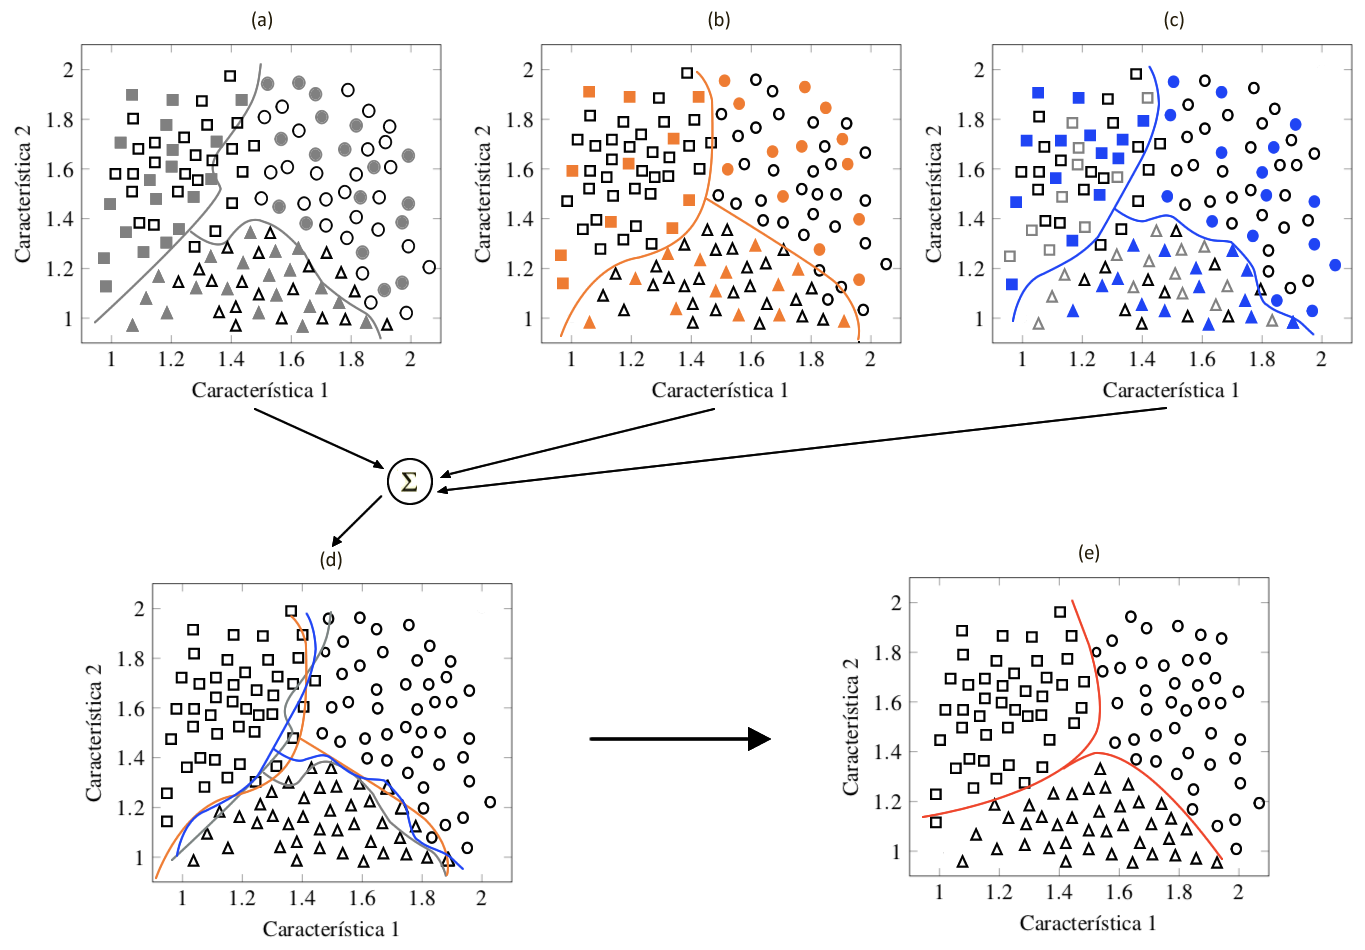
\includegraphics[scale=1.45]{Figuras/Cap4/ensemble.png}
    \begin{center}
    Fonte:
        O autor (2018), adaptado de \cite{zhang2012ensemble}.
    \end{center}
         
        \label{fig:ensemble}
\end{figure}

%FEITO
%\dbh{Sua abordagem de métodos ensemble está muito primitiva! Você precisa ler aqui uns 30 artigos, no mínimo, para melhorar este texto!}

\subsubsection{Teste do modelo}
\label{sec:meto1}

O algoritmo de teste de modelo foi pensado para testar os melhores modelos do algoritmo de seleção de modelo. Nesta fase de teste do modelo, foram utilizados os dados de teste, com objetivo de simular o comportamento real do modelo escolhido. cabe ressaltar que esse é o único momento em todo o trabalho em que os dados de teste são utilizado, a fim de simular o comportamento real do modelo.

O algoritmo proposto para o teste do modelo, neste trabalho, realiza dois \textit{ensemble}, executando várias redes (idealmente um número ímpar de redes), com modelos iguais e inicialização dos pesos diferentes.  Ao executar a previsão, as respostas de cada rede são ordenadas e é escolhida a mediana das respostas como resposta final. 
A técnica do \textit{ensemble} foi aplicada em dois contextos no teste do modelo:

\begin{enumerate}
    \item\textit{Ensemble} de modelo: tendo em vista os resultados da seleção de modelo, foram escolhidos os 7 modelos que apresentaram o menor desvio padrão para o \textit{Ensemble};
    \item \textit{Ensemble} de resultado: para cada modelo do \textit{ensemble} de modelo, são criadas 7 Redes Neurais com mesma arquitetura e inicialização diferente. Todas as 7 Redes Neurais são treinadas e testadas, onde o resultado do modelo passa ser a mediana dos resultados de todas as Redes. A mediana é uma medida mais robusta a aberrações do que a média, daí a sua adoção.
\end{enumerate}

Após executar os dois Ensembles, são obtidos os resultados que serão considerados para esse trabalho. No próximo capítulo serão apresentados os resultados do trabalho, obtidos com as metodologias aqui descritas.
\section{Resultados}

Como já foi adiantado no capítulo \ref{sec:algoritmos}, foram realizados 3 grandes avaliações de modelos para os 3 tipos de dados utilizados, que são: dados do valor do preço do Bitcoin, dados do valor do \textit{Google Trends} do termo Bitcoin e os dados do valor do preço do bitcoin e dados do valor do \textit{Google Trends} do termo Bitcoin combinados (concatenados em linha). Esta seção relatará cada um desses experimentos e mostra os resultados obtidos em cada base de dados


\subsection{Comparação dos resultados das três entradas testadas}

Como foi visto na seção \ref{sec:metodologia}, todas as 3 avaliações realizadas neste trabalho, utilizando as metodologias \ref{sec:meto0} e \ref{sec:meto1}, com as 3 bases de dados apresentados na seção \ref{sec:metobase}, serão apresentadas nas próximas seções.

\subsubsection{Resultado com a base de dados do Tipo 1}

Ao executar a metodologia \ref{sec:meto0} com os dados do Tipo 1, que contém apenas o valor do preço do Bitcoin, foram selecionados, ao final, 7 Modelos de Rede Neural a obterem os menores desvio padrão. Os 7 modelos vencedores da metodologia \ref{sec:meto0} são exibidos na Tabela \ref{tab:moto0-1}.

Todos os 7 modelos vencedores utilizaram a base de dados com com 5 amostras e PCA igual a 5, lembrando que o a frequência das amostras é diária. A arquitetura vencedora, que é a arquitetura que ficou na mediana dos valores, apresentou RMS igual a \textbf{24,6557\%}, Desvio padrão de \textbf{5,0190\%} e acurácia média de \textbf{56,6545\%}. Essa arquitetura foi a utilizada na metodologia \ref{sec:meto1}.

\begin{table}[!ht]
\centering

\caption{Tabela de avaliação de modelo dos dados do Tipo 1}
\label{tab:moto0-1}
\begin{tabular}{|M{0.2cm}|M{4cm}|M{1cm}|M{2cm}|M{1.6cm}|M{2cm}|M{1.5cm}|}
\hline
 &\#Neurônios na camada escondida&\#PCA &\#Amostras por linha&RMS (\%)&Desvio padrão (\%)&Acurácia (\%)\\\hline
 1&  1&  5&  5&  24,6357&  3,9080&  57,8748\\ 
 2&  9&  5&  5&  24,6498&  5,0229&  56,7289\\
 3&  7&  5&  5&  24,6515&  4,6648&  56,9145\\
 \textbf{4}&  \textbf{8}&  \textbf{5}&  \textbf{5}&  \textbf{24,6557}&  \textbf{5,0190}&  \textbf{56,6545}\\
 5&  4&  5&  5&  24,6760&  4,7606&  56,6483\\
 6&  5&  5&  5&  24,6773&  4,6635&  56,5674\\
 7&  2&  5&  5&  24,6818&  4,4030&  56,7106\\\hline
\end{tabular}
\begin{center}
	    Fonte: O autor (2018)
	\end{center}
\end{table}

Para executar a metodologia \ref{sec:meto1}, foram realizadas 7 testes da arquitetura vencedora, que podem ser vistos na Tabela \ref{tab:moto1-1}. O resultado final da base de dados do Tipo 1 foi de \textbf{50,7042\%}.

\begin{table}[!ht]
\centering

\caption{Tabela de teste dos dados do Tipo 1}
\label{tab:moto1-1}
\begin{tabular}{|M{0.4cm}|M{2cm}|}
\hline

 &Acurácia (\%)\\\hline
 1&48.826\\
 2&50,2347\\
 3&50,7042\\
 \textbf{4}&\textbf{50,7042}\\
 5&50,7042\\
 6&51.1737\\
 7&52.5822\\\hline
\end{tabular}
\begin{center}
	    Fonte: O autor (2018)
	\end{center}
\end{table}

\subsubsection{Resultado com a base de dados do Tipo 2}

Ao executar a metodologia \ref{sec:meto0} com os dados do Tipo 2, que contém apenas o valor do \textit{Google Trends} do Bitcoin, foram selecionados, ao final, 7 Modelos de Rede Neural a obterem os menores desvio padrão. Os 7 modelos vencedores da metodologia \ref{sec:meto0} são exibidos na Tabela \ref{tab:moto0-2}.

Todos os 7 modelos vencedores utilizaram a base de dados com com x amostras e PCA igual a x, com frequência de amostra diária. A arquitetura vencedora, que é a arquitetura que ficou na mediana dos valores, apresentou RMS igual a \textbf{24,7828\%}, Desvio padrão de \textbf{4,5962\%} e acurácia média de \textbf{52,5286\%}. Essa arquitetura foi a utilizada na metodologia \ref{sec:meto1}.

\begin{table}[!ht]
\centering
\caption{Tabela de avaliação de modelo dos dados do Tipo 2}
\label{tab:moto0-2}
\begin{tabular}{|M{0.2cm}|M{4cm}|M{1cm}|M{2cm}|M{1.6cm}|M{2cm}|M{1.5cm}|}
\hline
 &\#Neurônios na camada escondida&\#PCA &\#Amostras por linha&RMS (\%)&Desvio padrão (\%)&Acurácia (\%)\\\hline
 1&  1&  2&  4&  24,7250&  4,7261&  53,0957\\ 
 2&  2&  2&  4&  24.7503&  4,9895&  52,5204\\
 3&  3&  2&  4&  24,7772&  4,6581&  52,2155\\
 \textbf{4}&  \textbf{4}&  \textbf{2}&  \textbf{4}&  \textbf{24,7828}&  \textbf{4,5962}&  \textbf{52,5286}\\
 5&  10&  2&  4&  24,7891&  4,2942&  52,4477\\
 6&  6&  2&  4&  24,7912&  4,0864&  52,8628\\
 7&  12&  2&  4&  24,7975&  4,1099&  52,3636\\\hline
\end{tabular}
\begin{center}
	    Fonte: O autor (2018)
	\end{center}
\end{table}

Para executar a metodologia \ref{sec:meto1}, foram realizadas 7 testes da arquitetura vencedora, que podem ser vistos na Tabela \ref{tab:moto1-2}. O resultado final da base de dados do Tipo 2 foi de \textbf{49,2958\%}.

\begin{table}[!ht]
\centering

\caption{Tabela de teste dos dados do Tipo 2}
\label{tab:moto1-2}
\begin{tabular}{|M{0.4cm}|M{2cm}|}
\hline
 &Acurácia (\%)\\\hline
 1&48,8263\\
 2&48,8263\\
 3&48,8263\\
\textbf{4}&  \textbf{49,2958}\\
 5&49,2958\\
 6&49,7652\\
 7&49,7652\\\hline
\end{tabular}
\begin{center}
	    Fonte: O autor (2018)
	\end{center}
\end{table}

\subsubsection{Resultado com a base de dados do Tipo 3}

Ao executar a metodologia \ref{sec:meto0} com os dados do Tipo 3, que contém o valor do preço do Bitcoin e do valor do \texttt{Google Trends} do termo Bitcoin concatenados, foram selecionados, ao final, 7 Modelos de Rede Neural a obterem os menores desvio padrão. Os 7 modelos vencedores da metodologia \ref{sec:meto0} são exibidos na Tabela \ref{tab:moto0-3}.

Todos os 7 modelos vencedores utilizaram a base de dados com com 4 amostras e PCA igual a 2, com frequência de amostra diária. A arquitetura vencedora, que é a arquitetura que ficou na mediana dos valores, apresentou RMS igual a \textbf{24,7828\%}, Desvio padrão de \textbf{4,5962\%} e acurácia média de \textbf{52,5286\%}. Essa arquitetura foi a utilizada na metodologia \ref{sec:meto1}.

\begin{table}[!ht]
\centering

\caption{Tabela de avaliação de modelo dos dados do Tipo 3}
\label{tab:moto0-3}
\begin{tabular}{|M{0.2cm}|M{4cm}|M{1cm}|M{2cm}|M{1.6cm}|M{2cm}|M{1.5cm}|}
\hline
 &\#Neurônios na camada escondida&\#PCA &\#Amostras por linha&RMS (\%)&Desvio padrão (\%)&Acurácia (\%)\\\hline
 1&  3&  6&  6&  24,5493&  4,7034&  57,7263\\ 
 2&  2&  6&  6&  24,5499&  5,2139&  57,5297\\
 3&  13&  6&  6&  24,6325&  4,9916&  56,9421\\
 \textbf{4}&  \textbf{8}&  \textbf{6}&  \textbf{6}&  \textbf{24,6357}&  \textbf{5,1420}&  \textbf{56,5317}\\
 5& 10&  6&  6&  24,6402&  5,0183&  56,8247\\
 6&  6&  6&  6&  24,6405&  5,2531&  56,7097\\
 7&  9&  6&  6&  24,6409&  5,0773&  56,5769\\\hline
\end{tabular}
\begin{center}
	    Fonte: O autor (2018)
	\end{center}
\end{table}

Para executar a metodologia \ref{sec:meto1}, foram realizadas 7 testes da arquitetura vencedora, que podem ser vistos na Tabela \ref{tab:moto1-3}. O resultado final da base de dados do Tipo 3 foi de \textbf{53,9906\%}.

\begin{table}[!ht]

\centering

\caption{Tabela de teste dos dados do Tipo 3}
\label{tab:moto1-3}
\begin{tabular}{|M{0.4cm}|M{2cm}|}
\hline
 &Acurácia (\%)\\\hline
 4&53,0516\\
 1&53,5211\\
 2&53,0516\\
 3&553,9906\\
 \textbf{4}&\textbf{53,9906}\\
 5&54,4601\\
 6&54,9296\\
 7&55,8685\\\hline
\end{tabular}
\begin{center}
	    Fonte: O autor (2018)
	\end{center}
\end{table}

\subsection{Comparação do resultado com trabalhos anteriores}

O foco principal deste trabalho foi a comparação com trabalhos anteriores. Até a data deste trabalho, o único trabalho que havia apresentado uma metodologia e resultado para este problema, de predição dos valores futuros do Bitcoin, foi o trabalho \cite{mcnally2016predicting}. Por esse motivo este trabalho utilizou o mesmo intervalo de dados de \cite{mcnally2016predicting}, com objetivo de propor que os dados provenientes do \textit{Google Trends} pode ajudar aumentar a acurácia de um modelo de predição do valor do preço do Bitcoin. O resultado da comparação entre este trabalho e o \cite{mcnally2016predicting} pode ser encontrado na Tabela \ref{tab:compamatta2015}.

\begin{table}[!ht]
\centering

\caption[Tabela de comparação do resultado]{Tabela de comparação do resultado deste trabalho com o resultado do trabalho \cite{mcnally2016predicting}}
\label{tab:compamatta2015}
\begin{tabular}{|M{0.8cm}|M{2.4cm}|M{0.8cm}|M{2.6cm}|M{2.5cm}|}
\hline
 Tipo&Trabalho \cite{mcnally2016predicting} Acurácia (\%)&Tipo&Este trabalho Acurácia (\%)&Diferença (\%)\\\hline
 1&52,78&1&50,70&-2,08\\
 1&52,78&2&49,30&-3,48\\
 \textbf{1}&\textbf{52,78}&\textbf{3}& \textbf{53,99}&\textbf{+1,21}\\\hline
 
\end{tabular}
\begin{center}
	    Fonte: O autor (2018)
	\end{center}
\end{table}

\subsection{Comparação com o serviço Amazon Machine Learning}

Para fazer avaliações deste trabalho com outras metodolodias e técnicas de classificação binária, foi utilizado um serviço da Amazon, especificamente da AWS (\textit{Amazon Web Services}), que é o maior provedor de computação em nuvem do mundo, e oferece diversos serviços na area de Inteligência Artificial e \textit{Machine Learning}. Dentre os serviços disponíveis que permitem realizar a classificação binária, está o serviço chamado \textbf{Amazon Machine Learning}  \cite{amazonmachinelearning}, que foi utilizado com o objetivo de comparação de resultado com o modelo proposto neste trabalho.

O Amazon Machina Learning realiza basicamente 3 tipos de tarefas:

\begin{enumerate}
    \item Classificação binária: utilizando o algoritmo de Regressão logística, que usa a \textit{logistic loss function} somado com o gradiente descendente estocástico;
    \item classificação multi-classe: utilizando o alforitmo de Regressão logística multinomial, que usa a \textit{multinomial logistic loss} somado com o gradiente descendente estocástico;
    \item regressão: utilizando o algoritmo de Regressão, que usa a \textit{squared loss function} somado com o o gradiente descendente estocástico.
\end{enumerate}

Como este este trabalho se propõem a estudar um problema de classificação binária, foi utilizado a classificação binária Amazon Machine Learning. 

\subsubsection{Experimentos com o Amazon Machine Learning}

Para os experimentos com o Amazon Machine Learning, foram utilizados as mesmas bases de dados utilizadas na \ref{sec:meto1}, que foram as bases dos modelos vencedores provenientes da metodologia \ref{sec:meto0}. Foram utilizadas as configurações padrões e recomendadas pelo do serviço da Amazon, que utilizam 70\% dos dados para treinamento e 30\% para teste, separando os dados de maneira sequencial.

Para os dados vencedores do Tipo 1, que é a base de dados com apenas o valor do preço do Bitcoin com 5 amostras por linha e frequência de 1 dia. Essa configuração gerou resultado de 47,17\% 

Para os dados vencedores do Tipo 2, que é a base de dados com apenas o valor \textit{Google Trends} do Bitcoin com x amostras por linha e frequência de 1 dia. Essa configuração gerou resultado de 50,17\%.

Para os dados vencedores do Tipo 3, que é a base de dados com a concatenação de amostras o valor do preço do Bitcoin e do valor do \texttt{Google Trends} do termo Bitcoin, com 6, onde 3 são do valor do preço do Bitcoin e 3 \texttt{Google Trends} do termo Bitcoin amostras por linha e frequência de 1 dia, ou seja, essa base de dados representa dados de 3 dias. Essa configuração gerou resultado de 51,64\%.

A tabela \ref{tab:compamazon} apresenta o resultado da comparação 

\begin{table}[!ht]
\centering

\caption{Tabela Comparação do resultado da Amazon Machine Learning (AML) e da metodologia proposta neste trabalho}
\label{tab:compamazon}
\begin{tabular}{|M{0.8cm}|M{2.4cm}|M{2.6cm}|M{2.5cm}|}
\hline
 Tipo&AML Acurácia (\%)&Este trabalho Acurácia (\%)&Diferença (\%)\\\hline
 1&47,17&50,70&+3,53\\
 2&50,17&49,30&-0,87\\
 3&51,64&53,99&+2,35\\\hline
\end{tabular}
\begin{center}
	    Fonte: O autor (2018)
	\end{center}
\end{table}

\subsection{Teoria do mercado eficiente}

%Feito
%\dbh{eu esperava uma discussão muito mais profunda aqui, recheada de referências!}

A Teoria de mercado eficiente, proposta por \cite{malkiel1970efficient} em 1969, é uma Teoria que define uma mercado eficiente como aquele que sempre consegue refletir o preço do ativo de acordo quantidade de informações disponíveis desse ativo. De acordo com essa Teoria, é impossível alguém conseguir vencer o mercado, pois todas as informações disponíveis para precificar o ativo já estão disponíveis para todos os investidores. 

Na Teoria de mercado eficiente, como explica \cite{junior2004mercados}, sempre que uma informação nova fica disponível, automaticamente o mercado se adapta para ajustar o valor do preço do ativo, ou seja, o mercado sempre tende ao preço real de um ativo, ou valor intrínseco, com raras exceções \cite{jensen1978some}.

Dentro da teoria de mercado eficientes, como explicado em \cite{basu1977investment}, diversos estudo empíricos apontam que o preço refletem conjunto particular de informações  disponíveis sobre determinado ativo, sendo assim possível classificar 3 diferentes formas de eficiência:

\begin{itemize}
    \item Forma fraca: onde apenas informações do preço histórico dos ativos é levado em conta;
    \item forma semi-forte: onde a preocupação e se os preços vão se ajustar eficientemente a novas informações que surgirem, essas informações têm que ser, obviamente, públicas;
    \item forma forte: onde a preocupação é se mesmo que alguns investidores ou grupos (e.g., administradores de fundos de investimento) tenham informações privilegiadas relevantes para o preço, se o preço vai se adaptar a essas novas informações.
\end{itemize}

Essas classificações servem para identificar o montante de informação para cada uma das formas e conseguir distinguir quando elas falham. Cabe ressaltar os termos \textbf{preço real} ou \textbf{valor intrínseco} são aproximações, e não valores perfeitamente exatos. 

A teoria de mercado eficiente também é abordada em \cite{timmermann2004efficient} para a previsão de valores, mostrando que \textit{traders} (nome designado a investidores que compram e vendem ações em curto período de tempo, em geral no mesmo dia) tentam explorar o \textit{delay} que leva entre uma nova informação sobre um determinado ativo ficar disponível e o mercado atualizar o preço deste ativo.

Essa Teoria pode explicar a dificuldade encontrada tanto em \cite{mcnally2016predicting}, quanto neste trabalho em conseguir prever os valores do Bitcoin, mesmo com o uso do \textit{Google Trends}, que ajuda a encontrar comportamentos de manada dos investidores. O trabalho \cite{bartos2015does} avalia o ativo Bitcoin como um mercado eficiente, chegando na conclusão que os eventos disponíveis, tanto positivos, quanto negativos, influenciam diretamente o valor do Bitcoin, de modo extremamente rápido. Isso significa que o preço fica mais baixo durante eventos negativos, e permanecendo em alta durante eventos positivos. Também mostra o Bitcoin segue a formar padrão de oferta e demanda, podendo alterar bastante o preço do ativo.
\section{Conclusões}\label{conclusao}


Toda a implementação, junto com a documentação de como usar o códigos estão disponíveis no GitHub em \cite{repositorio}.

%\nocite{NBR6023,NBR6024,NBR6027,NBR6028,NBR10520,NBR14724,IBGE,CEFET_2007,CEFET_2014}



%@manual{CEFET_2014,
%address={Petr�polis (RJ)},
%organization={CELSO FEDERAL DE EDUCA��O TECNOL�GICO CELSO SUCKOW DA FONSECA. Campus Petr�polis. Coordena��o de %Trabalho %de Conclus�o de Curso},
%title={Manual para elabora��o de Trabalho de Conclus�o de Curso (TCC)},
%year={2014}
%}


%%% Bibliografia %%%
%\addcontentsline{toc}{section}{Refer�ncias}
%\bibliographystyle{apateste}

%\bibliographystyle{abnt-alf}
%{
\thispagestyle{empty}
\renewcommand{\refname}{REFERÊNCIAS}
\bibliography{bibliografia}
%}

\newpage

%\begin{appendices}
%%\renewcommand{\chaptername}{Ap�ndice}
%\section{Título do Apêndice} \label{ap:defesa}

\paragraph{Elemento que consiste em um texto ou documento elaborado pelo autor, com o intuito de complementar sua, sem prejuízo do trabalho. São identificados por letras maiúsculas consecutivas e pelos respectivos títulos.}
%\section{Título do Apêndice}

Documentação não elaborada pelo autor, ou elaborada pelo autor mas constituindo parte de outro projeto.
%%\include{apendiceD}
%\end{appendices}


\end{document}